\clearpage
\appendix



\clearpage

		\section{Broader Impact}
		We have presented an efficient framework for verifying fairness of linear classifiers. This work does not bear any negative societal impact. The sole purpose of our framework is to detect bias of machine learning models that are deployed in high-stake decision making. 
		

		\section{Background}
		
		\subsection{Fairness Metrics}
		In this section, we state the fairness metrics verified in this paper in further details.
		\subsubsection{Group Fairness.} Group fairness is categorized into three families: independence, separation and sufficiency, of which {\framework} verifies independence and separation metrics. 
		The independence metrics state that the predicition of the classifier should be independent of compound sensitive groups. Formally, independence notion specifies an equal PPV across all sensitive groups for a classifier $\alg$, i.e., $\Pr[\hat{Y} =1 | \mathbf{A} =  \mathbf{a}]  =  \Pr[\hat{Y} =1 | \mathbf{A} =  \mathbf{a}'] , \forall \mathbf{a}, \mathbf{a}' \in A$.
		Since satisfying independence exactly is hard, relaxations of independence fairness metrics, such as \textit{disparate impact} and \textit{statistical parity}~\cite{dwork2012fairness,feldman2015certifying}, are proposed. 
		
		\textit{Disparate impact} (DI)~\cite{feldman2015certifying} measures the ratio of PPVs between the most favored group and least favored group, and prescribe it to be close to $1$. Formally, a classifier satisfies $(1 - \epsilon)$-disparate impact if, for $\epsilon \in [0,1] $,
		\[
		\min_{\mathbf{a}} \Pr[\hat{Y} =1 | \mathbf{A} =  \mathbf{a}]  \ge (1 - \epsilon) \max_{\mathbf{a}'} \Pr[\hat{Y} =1 | \mathbf{A} =  \mathbf{a}'].
		\]
		Another popular relaxation of independence metrics  is \textit{statistical parity} (SP) that measures the difference of PPV among sensitive groups, and prescribe this to be near zero. Formally, an algorithm satisfies $\epsilon$-statistical parity if, for $\epsilon \in [0,1] $, 
		\[
		\max_{\mathbf{a}, \mathbf{a}'}|\Pr[\hat{Y} =1 | \mathbf{A} = \mathbf{a}] - \Pr [\hat{Y} = 1| \mathbf{A} = \mathbf{a}']| \le \epsilon.
		\]
		For both disparate impact and statistical parity, lower value of $\epsilon$ indicates higher group fairness of the classifier $\alg$. 
		
		
		In the \textit{separation (or classification parity)} notion of fairness, the predicted label $\hat{Y}$ of a classifier $\alg$ is independent of the sensitive features $\sensitive$ given the class labels $Y$. In case of binary classifiers, a popular separation metric is \textit{equalized odds} (EO)~\cite{hardt2016equality} that computes the difference of false positive rates (FPR) and the difference of true positive rates (TPR) among all compound sensitive groups. 
		Lower value of equalized odds indicates better fairness.
		A classifier $\alg$ satisfies $\epsilon$-equalized odds if, for all compound sensitive groups $\mathbf{a}, \mathbf{a}' \in A$,
		$ \max_{\mathbf{a}, \mathbf{a}'} |\Pr[\hat{Y} =1 |\mathbf{A}= \mathbf{a}, Y= 0  ] - \Pr [\hat{Y} = 1|\mathbf{A}= \mathbf{a}', Y = 0]| \le \epsilon, $ and $
		\max_{\mathbf{a}, \mathbf{a}'}|\Pr[\hat{Y} =1 |\mathbf{A}= \mathbf{a}, Y= 1  ] - \Pr [\hat{Y} = 1|\mathbf{A}= \mathbf{a}', Y = 1]| \le \epsilon.
		$
		
		
		
		\subsubsection{Path-specific Causal Fairness.}
		Let $ \mathbf{a}_{\max}  \triangleq \argmax_{ \mathbf{a}} \Pr[\hat{Y} =1 |\mathbf{A}=  \mathbf{a}] $. We consider mediator features $ \mediator \subseteq \nonsensitive $ sampled from the conditional distribution $ {\mathcal{Z}_{|\mathbf{A} = \mathbf{a}_{\max}}} $. This emulates the fact that mediator variables have the same sensitive features $ \mathbf{a}_{\max} $.  For $ \epsilon \in [0,1] $,  path-specific causal fairness is defined as 
		$
		\max_{\mathbf{a}, \mathbf{a}'} |\Pr[\hat{Y} = 1 | \sensitive =  \mathbf{a}, \mediator] - \Pr[\hat{Y} = 1 | \sensitive = \mathbf{a}', \mediator ]| \le \epsilon
		$.
		
		Therefore, PCF constrains that $ \hat{Y} $ is not directly dependent of $ \sensitive $ while $ \sensitive $ may indirectly affects $ \hat{Y} $ only through $ \mediator $. PCF is a variation of counterfactual fairness and causal fairness without mediator features~\cite{bastani2019probabilistic}. 
		
		
	
		
		\begin{example}
			Following~\cite{bastani2019probabilistic}, we consider a classifier that decides the hiring of employees based on three features: gender (sensitive), years of experience (non-sensitive), and college-participation (mediator). It is practical to consider that gender $ \in $ \{male, female\} can affect the college-participation of individuals, and all three features are determining factors for the hiring process. Let `male' be the most favored group by the classifier, for instance. Path-specific causal fairness (PCF) ensures that a female candidate should be given a job offer with similar probability as a male candidate (by constraining $ \epsilon \approx 0 $). She,  however,  went to (participated in) college as if she were a male candidate while other non-mediator features such as  `years of experience' are the same.  Therefore, PCF measures the effect of gender on job offer, but ignores the effect of gender on whether candidates went to college.
		\end{example}	
		
	
%		\newpage
		\section{Proofs of Theoretical Results}
		\iffalse
		\begin{lemmarep}
			$ S(B,\tau) $ does not rely on the order of $\mathbf{B}$.\footnote{\blue{This is the rectified version of Lemma~\ref{lm:property-subset-sum}. We note that this correction does not change any claim in Section~\ref{sec:fvgm} except the proposed heuristic in Section~\ref{sec:dp_formulation}, which we address in final version of the paper.}}
		\end{lemmarep}
		\begin{proof}
		The quantifiers in $\mathbf{B}$ can be either universal, existential, or random. The sum of weights for existential and universal variables in $\mathbf{B}$ are calculated as $ w_{\exists} =  \sum_{i|q_i = \exists} \max\{w_i, 0\}$ and  $ w_{\forall} =  \sum_{i|q_i = \forall} \min\{w_i, 0\}  $, respectively by following Eq.~\eqref{eq:dp_recurse}.   Since the contributions of $ w_\exists $ and $ w_\forall $ in $S(B,\tau)$ are fixed, it suffices to prove that $ S(B,\tau) $ does not rely on the order of \textit{random variables} in $\mathbf{B}$. 
		
		Let  $ \tau' =  \tau - w_\exists - w_\forall$ be the revised threshold for random variables $ B' = \{B_i | q_i = \R\} \subseteq\mathbf{B}$. Then $ S(B,\tau) $ is equivalent to solving $ S(B', \tau') $, and we show that $ S(B', \tau') $ does not rely on the order of $ B' $.
		
		We consider an indicator function $ f_w(i, b) $ that outputs the weight of $ B_i $ based on its assignment $\mathbf{B}$. 
\begin{align*}
		f_w(i, b) = \begin{cases}
	w_i &\text{ if }\mathbf{B}= 1, \\
	0 &\text{ if }\mathbf{B}= 0.
	\end{cases}
\end{align*}
		Let $ \sigma \in \{0,1\}^{|B'|} $ be a vector of  assignments of variables in $ B' $. Then, $ S(B', \tau') $ is computed as
		\[ S(B', \tau') = \sum_{\sigma \in \{0,1\}^{|B'|}}  \mathds{1}[\sum_{i=1}^{|B'|} f_w(i, \sigma_i) \ge \tau'] \prod_{i=1}^{|B'|}\Pr[B_i = \sigma_i]. \]
		 The aforementioned equation represents a stochastic subset-sum problem, where for each assignment $ \sigma $, we compute the decision version of the subset-sum problem corresponding to $ \sigma $ and multiply with probabilities of random-variables. We observe that $ S(B',\tau') $ does not rely on the order of $ B' $, because both multiplication and addition operations are commutative for real numbers. 
			\end{proof}
		\iffalse
		\begin{lemmarep}
			Let $ Q = \{q_i\} $ be the set of quantifiers of $\mathbf{B}$. If $ |Q| = 1$, then $ Q $ is called homogeneous, and otherwise $ Q $ is called heterogeneous. If $ Q $ is homogeneous, then $ S(B,\tau) $ does not rely on the order of $\mathbf{B}$. Otherwise, $ S(B, \tau) $ is order-specific to $\mathbf{B}$.
		\end{lemmarep}
	
		\begin{proof}
			When $ |Q|  = 1 $, all variables in $\mathbf{B}$ are either existential, universal or random. When all variables are existential, $ S(B,\tau) $ is solved linearly in $ |B| $ as $ S(B, \tau) = \mathds{1}[\sum_i \max\{w_i, 0\} \ge \tau] $. Similarly, when all variables are universal, $ S(B, \tau) = \mathds{1}[\sum_i \min\{w_i, 0\} \ge \tau] $. In both cases,  the sum of $ |B| $ integers does not depend on the order of integers.
			
			We consider an indicator function $ f_w(i, b) $ that outputs the weight of $ B_i $ depending on its assignment $\mathbf{B}$. 
			\[
			f_w(i, b) = \begin{cases}
			w_i \text{ if }\mathbf{B}= 1 \\
			0 \text{ if }\mathbf{B}= 0
			\end{cases}
			\]
			Let $ \sigma \in \{0,1\}^{|B|} $ be a vector of  assignments of $\mathbf{B}$. When all variables are random, $ S(B, \tau) $ is computed as
			\[ S(B, \tau) = \sum_{\sigma \in \{0,1\}^{|B|}}  \mathds{1}[\sum_{i=1}^{|B|} f_w(i, \sigma_i) \ge \tau] \prod_{i=1}^{|B|}\Pr[B_i = \sigma_i], \]
			which also does not rely on the order of $\mathbf{B}$. Therefore, if $ Q $ is homogeneous, $ S(B,\tau) $ does not rely on the order of $\mathbf{B}$.
			
			
			\red{Lemma is not correct}
			
		\end{proof}
	\fi
	
		\begin{lemmarep}
			The decision version of the fairness verification problem for linear classifiers is in $\mathrm{NP^{PP}}$.
		\end{lemmarep}
	
		\begin{proof}
			
			\textbf{Case 1: Subset-sum problem is $ \mathrm{NP} $-complete by a reduction to $ 3 $-SAT.}
			
			We show that subset-sum problem is a $ \mathrm{NP} $-complete problem. In particular, we show that computing $ \sum_{i} w_iB_i = \tau $ for $ B_i \in\mathbf{B}$ is $ \mathrm{NP} $-complete through a reduction to $ 3 $-SAT~\cite{kleinberg2006algorithm}. $ 3 $-SAT problem computes a satisfying assignment of  a CNF formula, say $ \phi $, defining over $ n $ variables $ X_1, \dots, X_n $ and $ m $ clauses $ C_1, \dots, C_m $ where each clause has three literals. We start by defining two integer weights $ a_i $ and $ b_i $ associated with each variable $ X_i $, where including $ a_i $ corresponds to assigning $ X_i $ to true and including $ b_i $ corresponds to assigning $ X_i $ to false. We compute $ a_i $ and $ b_i $ in the following. 
			\begin{align*}
				&a_i = 10^{m+i} + \sum_{j|X_i \in C_j} 10^j\\
				&b_i = 10^{m+i} + \sum_{j|\neg X_i \in C_j} 10^j
			\end{align*}
			
			We construct a subset-sum problem of $ 2n $ variables with weights $ W =  \cup_{i=1}^n\{a_i, b_i\} $. Concretely, let $\mathbf{B}= \{B_{1,1}, B_{1,2}, \dots, B_{n,1}, B_{n,2}\} $ be the set of variables such that $ w(B_{i,1}) = a_i $ and $ w(B_{i,2}) = b_i $ and our goal is to compute an assignment of $\mathbf{B}$ such that $ \sum_{i} w(B_{i,1})B_{i,1} + w(B_{i,2})B_{i,2} = \tau $.
			
			
			Let $ \sigma $ be a satisfying assignment of $ 3 $-SAT formula $ \phi $. Given the assignment $\sigma$, we consider a \textit{solution} of the subset-sum problem by assigning $ B_{i, 1} = 1 $ and $ B_{i, 2} = 0 $ whenever $ \sigma(X_i) = 1 $, and $ B_{i, 1} = 0 $ and $ B_{i, 2} = 1 $ whenever $ \sigma(X_i) = 10 $. Intuitively, 
			we consider a subset of weights from $ W $ by including 
			 $ a_i $ if $ X_i $ is true and otherwise we include $ b_i $.  
			 The sum of \textit{included} weights has following properties. 
			\begin{itemize}
				\item  the sum has $ 1 $ in leftmost $ n $ digits, corresponding to $ 10^{m+i} $ for $ i = 1, \dots, n $ as we include one of $ a_i $ or $ b_i $ for each $ i $. 
				\item the sum has $ 1, 2 $, or $ 3 $ in the next $ m $ digits. The digit $ 10^j $ is the number of true literals in clause $ C_j $ and it is non-zero since $ \sigma $ satisfies each clause in  $ \phi $.
				\item $ 0 $ in the rightmost digit.
			\end{itemize}
		
			In the subset-sum problem, we set the threshold $ \tau = \sum_{i=1}^n 10^{m+i} + 3 \sum_{j=1}^m 10^j $. We additionally consider integer weights $ c_j =  d_j = 10^j $, which will be added to $ W $ as discussed next. For brevity of presentation, we are not assigning Boolean variables in $\mathbf{B}$ for additional weights $ c_j $ and $ d_j $.
			 We then prove that  $ \sum_{i} w(B_{i,1})B_{i,1} + w(B_{i,2})B_{i,2} = \tau $ if and only if $ \phi $ is satisfiable. 
			
			\begin{itemize}
				\item If $ \phi $ is satisfiable, then we select weights $  a _i $ if $ \sigma(X_i) = 1 $, else $ \mathbf{B}_i $. As discussed above, the sum of selected weights has leftmost $ n $ digits of $ \tau $ correct. To make remaining digits correct, we may need to add both of $ c_j $ and $ d_j $, one of $ c_j $ and $ d_j $, or none of $ c_j $ and $ d_j $ depending  if the digit $ 10^j $ in the sum is $ 1,2, $ or $ 3 $. We emphasis that this addition is deterministic as it relies on the number of true literals in $ C_j $ for the assignment $ \sigma $. Thus, for a satisfying assignment of $ 3 $-SAT, there exists a solution of the subset-sum problem. 
				
				\item Finally, we prove that a solution of the subset-sum problem corresponds to a satisfying assignment of $ \phi $.  First we observe that in any digit $ 10^k $, for $ k \le m $, there are at most five weights with $ 1 $ in digit $ 10^k $: the three literals corresponding to clause $ k $ and $ c_k $ and $ d_k $ (otherwise when $ k > m $, there are at most $ 2 $  weights with $ 1 $ in digit $ 10^k $).  Since there are at most $ 5 $ ones in any position, a subset of these weights will not cause any carries in addition. Hence, we can only get a total of $ \tau $ by including the right number of $ 1 $s in any digit. To do this, one needs to include exactly one of $ a_i $ and $ b_i $, and the corresponding truth assignment $ \sigma $ needs to satisfy $ \phi $ so that in each position $ 1 \le j \le m $, we get at least one $ 1 $ in digit $ 10^j $. We can then add $ c_j $ and $ d_j $ to increase the sum of weights to $ \tau $, as discussed previously. This, for a solution of the subset-sum problem, there is a corresponding satisfying assignment of $ 3 $-SAT
			\end{itemize}
		
		
			In the above analysis, the construction of $ a_i $ and $ b_i $ has polynomial complexity with respect to $ n $ and $ m $. Therefore, the subset-sum problem $ \sum_{i} w(B_{i,1})B_{i,1} + w(B_{i,2})B_{i,2} = \tau $ and equivalently, $ \sum_{i} w_iB_i = \tau $ is $ \mathrm{NP} $-complete because $ 3 $-SAT is also $ \mathrm{NP} $-complete. We further claim that computing $ \sum_{i} w_iB_i \ge \tau $ is at least as hard as computing $ \sum_{i} w_iB_i = \tau $, which is required for analyzing the complexity of stochastic subset-sum problem, as discussed next.
			
			\textbf{Case 2: Stochastic subset-sum problem is $ \mathrm{PSPACE} $-complete by a reduction to $ 3 $-SSAT.}
			
			We observe that a $ 3 $-SSAT formula that is based on a $ 3 $-SAT formula $ \phi $ and an additional specification of quantifiers for each variable in $ \phi $. Concretely, we define a $ 3 $-SSAT formula $$ \Phi \triangleq (\{q(X_i)\}_{i=1}^{n}, \phi) \text{ , where } q(X_i) \in \{\exists, \forall, \R^{p}\} .$$ To analyze the complexity of a stochastic subset-sum problem, we discuss a procedure in the following that is based on a polynomial reduction to $ 3 $-SSAT.
			
			
			We apply the aforementioned construction procedure ($ 3 $-SAT to subset-sum problem) to translate  a $ 3 $-SSAT formula to a stochastic sub-set sum problem. In particular, for each quantified variable in $ \phi $, we now discuss the quantifier of variables in the stochastic subset-sum problem.  If $ X_i $ is $ \exists $ (resp.\ $ \forall $) quantified, associated $ B_{i,1} $ and $ B_{i,2} $ are also $ \exists $ (resp.\ $ \forall $) quantified. Moreover, if $ X_i $ is randomized ($ \R^{p_i} $) quantified with $ p_i = \Pr[X_i = 1] $, then both $ B_{i,1} $ and $ B_{i,2} $ are randomized quantified with probability $ \Pr[B_{i,1}] = p_i $ and $ \Pr[B_{i,2}] = 1 - p_i $. Since the decision version of $ 3 $-SSAT is $ \mathrm{PSPACE} $-complete~\cite{littman2001stochastic}  and the presented reduction procedure has polynomial complexity, the decision version of stochastic subset-sum if also $ \mathrm{PSPACE} $-complete. 
			
			\textbf{Case 3: Fairness verification for linear classifiers is in
			$\mathrm{NP^{PP}}$ by a reduction to E-MAJSAT.}
		
		
			
			E-MAJSAT is a specific quantifier arrangement of SSAT problems where existential (or universal) variables appear before random variables. Formally, a E-MAJSAT formula 
			$$ \Phi =  (\{q(X_1) = \exists,\cdots,q(X_i) =\exists, q(X_{i+1}) =\R^{p_{i+1}}, \cdots, q(X_n) = \R^{p_{n}} \}, \phi).$$ The decision version of E-MAJSAT problem has complexity in $\mathrm{NP^{PP}}$~\cite{littman2001stochastic}. Furthermore, the decision version of SSAT problems with universal quantifiers followed by random-quantifiers are also in $\mathrm{NP^{PP}}$ as this a dual problem of E-MAJSAT~\cite{littman2001stochastic}. 
			In Section~\ref{sec:fvgm}, we present fairness verification of linear classifiers defined over Boolean variables using a formulation of stochastic subset-sum problem. Similar to E-MAJSAT,  existential (or universal) variables appear before random variables in our formulation.  Thus, the decision version of fairness verification of linear classifiers is in $\mathrm{NP^{PP}}$.
			\iffalse 
			\red{We further highlight that verification of linear classifiers on continuous real-valued variables is at least as hard as verifying classifiers on Boolean variables.}\fi
		\end{proof}
		\fi
	
	
	
	
		
		\begin{lemmarep}
			Let $ n' $ be the number of existential and universal variables in $ \mathbf{B} $. Let $ w_{\exists} = \sum_{B_i \in \mathbf{B} | q_i = \exists} \max\{w_i, 0\}$  and $ w_{\forall} = \sum_{B_i \in \mathbf{B} | q_i = \forall} \min\{w_i, 0\}$ be the considered sum of weights of existential and universal variables, respectively. We can exactly solve {\stochastic} using dynamic programming with time complexity $ \mathcal{O}((n - n')(\tau + |w_{neg}| - w_{\exists} - w_{\forall}) + n') $. The space complexity is  $ \mathcal{O}((n - n')(\tau + |w_{neg}| - w_{\exists} - w_{\forall})) $.
		\end{lemmarep}
	
		\begin{proof}
			\textbf{Case 1: All $n$ variables in $\mathbf{B}$ have randomized quantifiers.}
			
			At step-$i$ of the dynamic programming (Eq.~\eqref{eq:dp_recurse}), we modify the residual threshold of that step, namely $\tau_i$, either by subtracting $w_i$ or by retaining it.
			Now, we observe that the residual threshold $\tau_i$ for any $i \in \lbrace1,\ldots,n\rbrace$ will be in $[0, \tau+|w_{neg}|]$. This holds because if $\tau_i$ crosses these bounds, the dynamic programming is terminated as shown in Equation~\eqref{eq:dp_terminus}.
			Since all weights of $\{w_i\}_{i=1}^{n}$ are integers, the maximum number of values that the residual threshold can take, is $ (\tau + |w_{neg}|) $.
			Thus, we need to store at most $ n(\tau + |w_{neg}|)$ values in the memory for performing dynamic programming with $n$ variables and $ (\tau + |w_{neg}|) $ number of possible weights.
			Thus, the space complexity  is $ \mathcal{O}(n(\tau + |w_{neg}|)) $.  
			
			In order to construct the dynamic programming table, we have to call the $\mathsf{dp}$ function $ \mathcal{O}(n(\tau + |w_{neg}|)) $ times, in the worst-case.
			Thus, the time complexity of our method is $ \mathcal{O}(n(\tau + |w_{neg}|) $.
			
			
			\textbf{Case 2: $n'$ variables have existential or universal quantifiers and $n-n'$ variables have randomized quantifiers in $\mathbf{B}$.}

			According to Eq.~\eqref{eq:dp_recurse}, $ w_\exists $ and $ w_\forall $ are the fixed weights of all existential and universal variables, respectively. Therefore, we need to consider at most $ \tau + |w_{neg}| -  w_\exists - w_\forall $ values of residual weights for random variables. By applying analysis in Case 1, the space and time complexity is derived as $ \mathcal{O}((n - n')(\tau + |w_{neg}| - w_{\exists} - w_{\forall})) $. 
			
			We note that there is an additional time complexity of $ \mathcal{O}(n') $ for existential and universal variables in Eq.~\eqref{eq:dp_recurse}. Thus the time complexity becomes $ \mathcal{O}((n - n')(\tau + |w_{neg}| - w_{\exists} - w_{\forall}) + n') $. We, however, do not require to store any entry for existential and universal variables in $ \mathsf{dp} $  function and thus, the space complexity remains the same as $ \mathcal{O}((n - n')(\tau + |w_{neg}| - w_{\exists} - w_{\forall})) $.
		\end{proof}
	
		\begin{lemmarep}
			Let $ \mathbf{V} \subseteq \mathbf{B} $ be the set of vertices in the Bayesian network and $ n'' $ be the number of existential and universal variables in $ \mathbf{B} \setminus \mathbf{V} $. Let $ w'_{\exists} = \sum_{B_i \in \mathbf{B} \setminus \mathbf{V} | q_i = \exists} \max\{w_i, 0\}$  and $ w'_{\forall} = \sum_{B_i \in \mathbf{B} \setminus \mathbf{V} | q_i = \forall} \min\{w_i, 0\}$ be the sum of considered weights of existential and universal variables, respectively that only appear in $ \mathbf{B} \setminus \mathbf{V} $. To exactly compute {\stochastic} with correlated variables in dynamic programming approach,  time complexity is $ \mathcal{O}(2^{|\mathbf{V}|} + (n - n'' - |\mathbf{V}|)(\tau + |w_{neg}| - w'_{\exists} - w'_{\forall}) + n'') $ and space complexity is $ \mathcal{O}((n - n'' - |\mathbf{V}|)(\tau + |w_{neg}| - w'_{\exists} - w'_{\forall})) $.
		\end{lemmarep}	
	
	
		\begin{figure}
	\begin{center}
		\subfloat[]{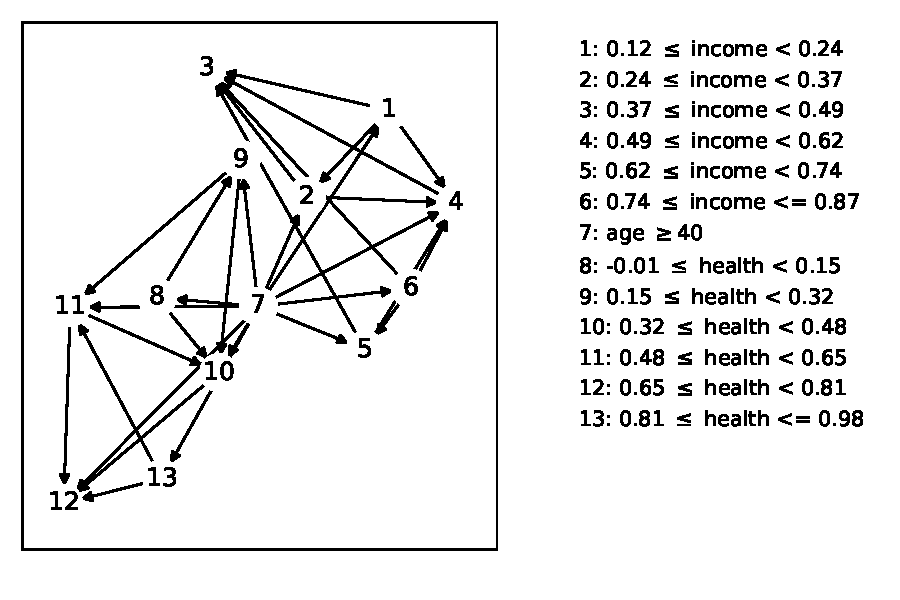
\includegraphics[scale=0.5]{figures/fairness/fvgm/synthetic_example_BN}\label{fairness_fvgm_fig:synthetic_bn}}
		
		\subfloat[]{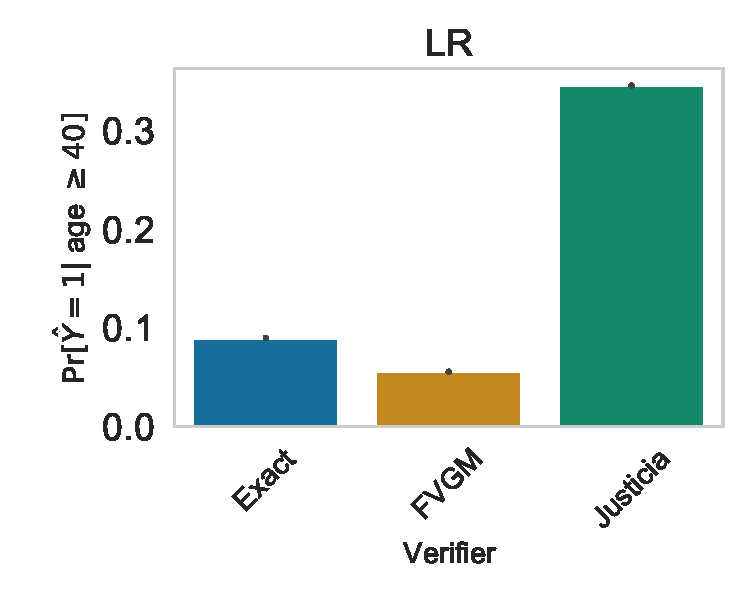
\includegraphics[scale=0.4]{figures/fairness/fvgm/sanity_ppv_max_PPV_LR}\label{fairness_fvgm_fig:synthetic_ppv_max_LR}}
		\subfloat[]{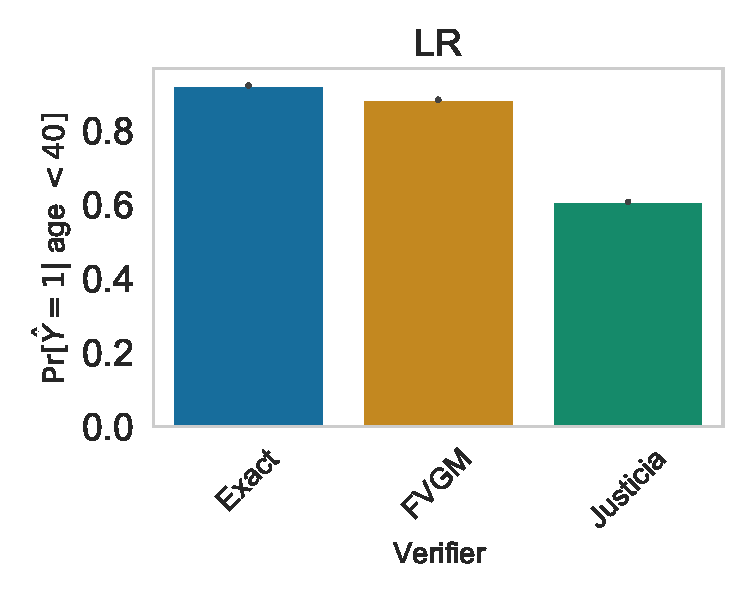
\includegraphics[scale=0.4]{figures/fairness/fvgm/sanity_ppv_min_PPV_LR}\label{fairness_fvgm_fig:synthetic_ppv_min_LR}}
		
		\subfloat[]{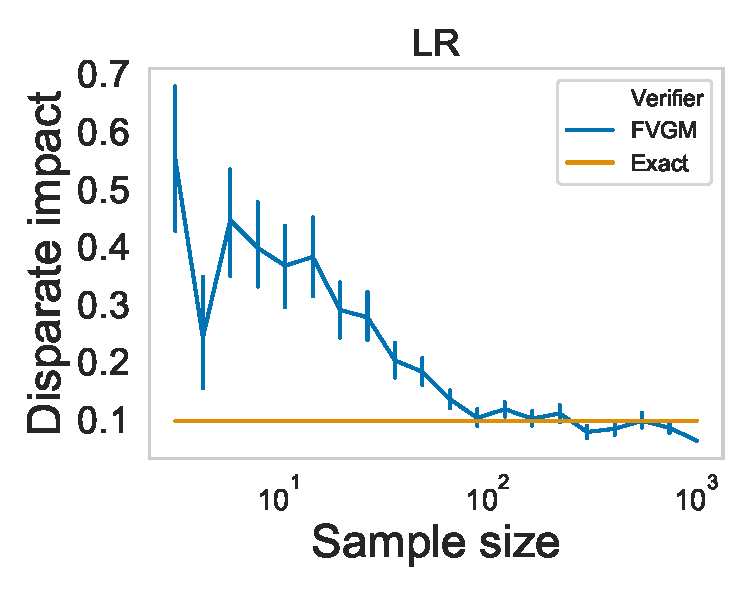
\includegraphics[scale=0.4]{figures/fairness/fvgm/sanity_sample_size_DI_LR}\label{fairness_fvgm_fig:synthetic_sample_size_LR_DI}}
		\subfloat[]{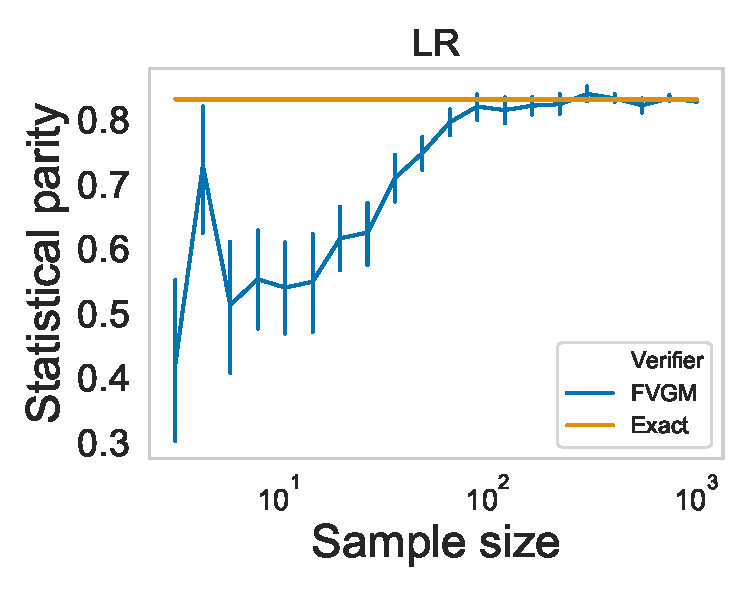
\includegraphics[scale=0.4]{figures/fairness/fvgm/sanity_sample_size_SPD_LR}\label{fairness_fvgm_fig:synthetic_sample_size_LR_SPD}}
	\end{center}
	
	\caption[Accuracy of {\fvgm} on logistic regression classifier]{
		Measuring accuracy of different fairness verifiers for Example~\ref{fairness_justicia_example:intro} on logistic regression classifier.}
	\label{fairness_fvgm_fig:synthetic_results}
\end{figure}


\begin{figure}
	\begin{center}
		\subfloat{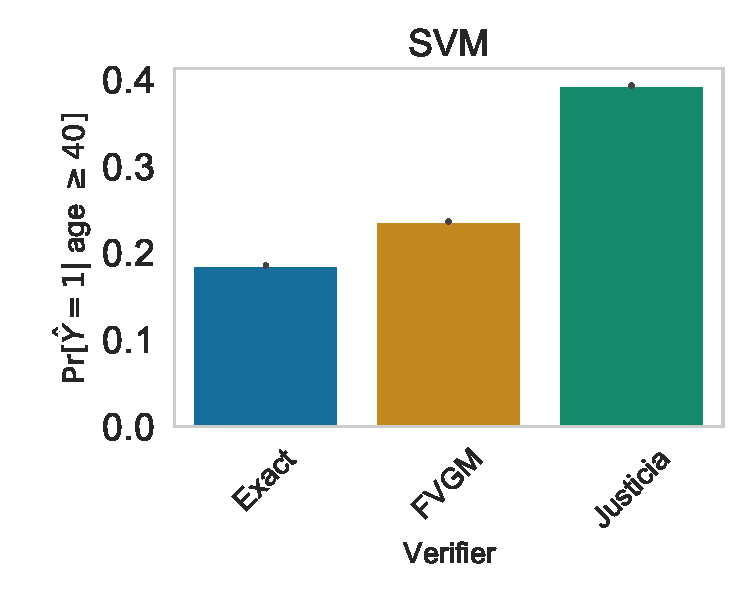
\includegraphics[scale=0.4]{figures/fairness/fvgm/sanity_ppv_max_PPV_SVM}}
		\subfloat{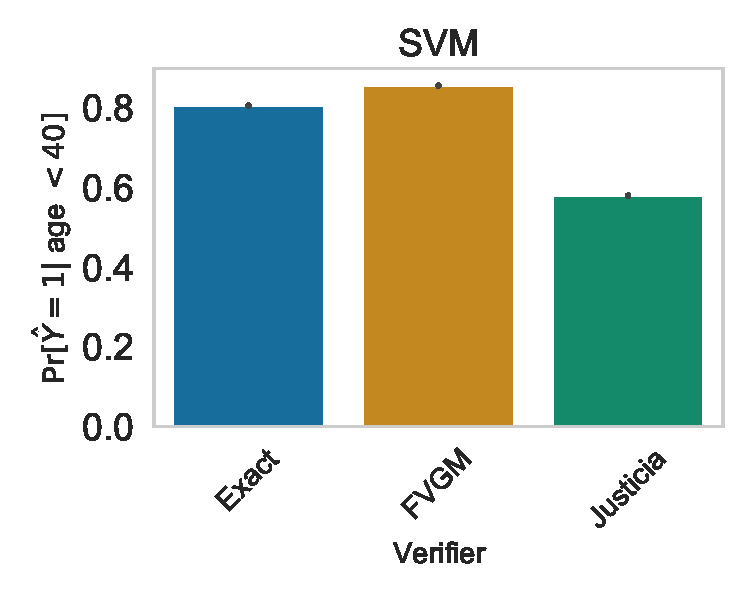
\includegraphics[scale=0.4]{figures/fairness/fvgm/sanity_ppv_min_PPV_SVM}}\\
		\subfloat{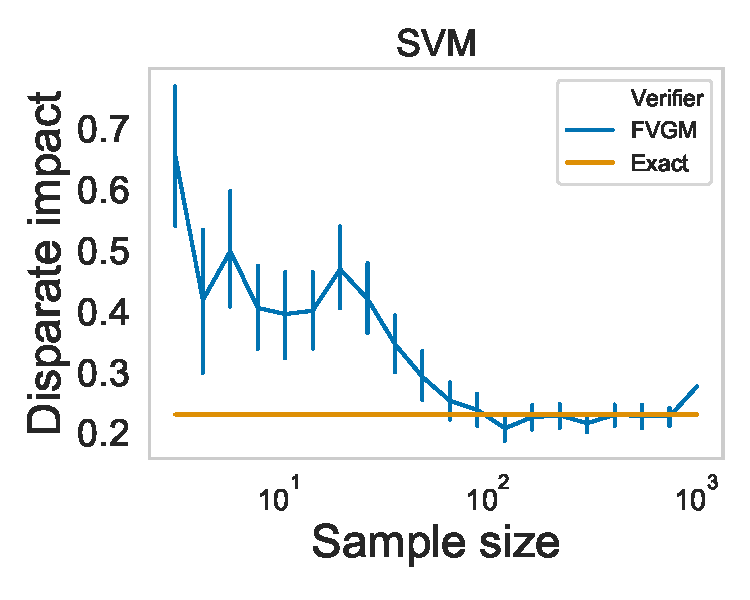
\includegraphics[scale=0.4]{figures/fairness/fvgm/sanity_sample_size_DI_SVM}}
		\subfloat{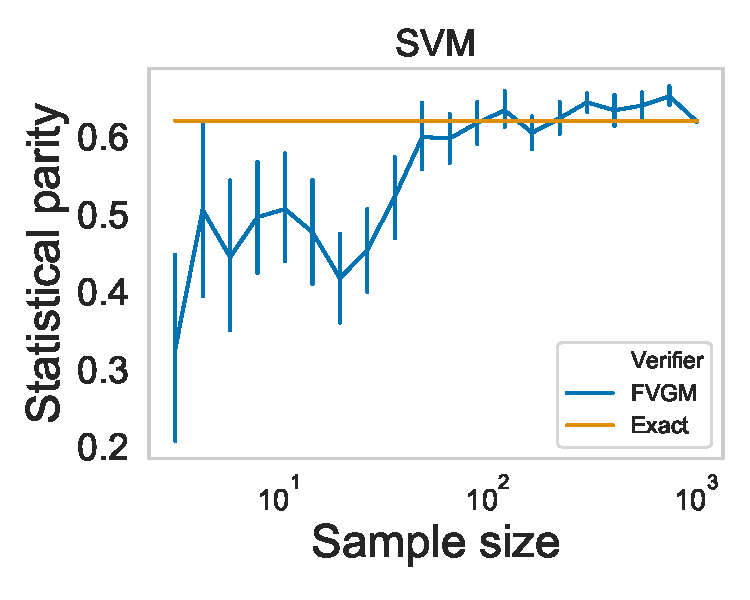
\includegraphics[scale=0.4]{figures/fairness/fvgm/sanity_sample_size_SPD_SVM}}
		
	\end{center}
	
	\caption[Accuracy of {\fvgm} on SVM classifier]{
		Measuring accuracy of different fairness verifiers for Example~\ref{fairness_justicia_example:intro} on SVM classifier.}
	\label{fairness_fvgm_fig:synthetic_results_SVM}
\end{figure}



	
	
	

	
		\begin{proof}
			We first separate analysis of space and time complexity for variables in $ \mathbf{V} $ and in $\mathbf{B}\setminus \mathbf{V} $. For each Boolean variable in $ \mathbf{V} $, we enumerate all assignments, which has time complexity of $ 2^{|\mathbf{V}|} $ and there is no space complexity as discussed in Section~\ref{sec:dp_with_BN}. 
			
			
			For variables in $\mathbf{B}\setminus \mathbf{V} $, we apply analysis from  Lemma~\ref{lemma:complexity_sss}, where we consider $ (n - n'' - |\mathbf{V}|) $ random variables, $ n'' $ existential/universal variables, and residual weights can take at most $ (\tau + |w_{neg}| - w'_{\exists} - w'_{\forall}) $ values. Hence, time complexity is $ \mathcal{O}((n - n'' - |\mathbf{V}|)(\tau + |w_{neg}| - w'_{\exists} - w'_{\forall}) + n'') $, and space complexity is $ \mathcal{O}((n - n'' - |\mathbf{V}|)(\tau + |w_{neg}| - w'_{\exists} - w'_{\forall})) $ 
			
			Combining two cases, overall time complexity is $ \mathcal{O}(2^{|\mathbf{V}|} + (n - n'' - |\mathbf{V}|)(\tau + |w_{neg}| - w'_{\exists} - w'_{\forall}) + n'') $ and space complexity is $ \mathcal{O}((n - n'' - |\mathbf{V}|)(\tau + |w_{neg}| - w'_{\exists} - w'_{\forall})) $. 
		\end{proof}
		
	
%	\newpage	
	\section{Extended Experimental Evaluations}
	\label{appendix:experiments}
	Each experiment is performed on Intel Xeon E$ 7-8857 $ v$2 $ CPUs with $ 16 $GB memory, $ 64 $bit Linux distribution based on Debian OS and clock speed $ 3 $ GHz. In the following, we discuss extended experimental results.



	\subsection{Accuracy Comparison Among Different Verifiers}
	We have considered a synthetic problem for comparing accuracy among different verifiers. For Example~\ref{example:intro}, we consider `age $ \ge 40 $' as a Bernoulli random  variable with probability $ 0.5 $. For `income' feature ($ I $), we consider two Gaussian distributions $ \Pr[I | \text{age} \ge 40] \sim \mathcal{N}(0.6, 0.1) $ and $ \Pr[I | \text{age} < 40] \sim \mathcal{N}(0.4, 0.1) $ separated by two age groups. Moreover, for `fitness' feature ($ F $), we consider two Gaussian distributions $ \Pr[F | \text{age} \ge 40] \sim \mathcal{N}(0.7, 0.1) $ and $ \Pr[F | \text{age} < 40] \sim \mathcal{N}(0.3, 0.1) $. On this data, the trained LR and SVM classifier has decision boundary as $ 7.26I + 7.4F - 1.34A \ge 6.62 $ and $ 9.37I + 9.75F - 0.34A \ge 9.4 $, respectively.
	
	
	In Figure~\ref{fig:synthetic_bn} we show the Bayesian Network on discretized features, in particular for income and fitness features. In Figure~\ref{fig:synthetic_ppv_max_LR} \ to Figure~\ref{fig:synthetic_ppv_min_SVM}, we show PPVs of different classifiers computed by different verifiers, where  {\framework} outputs closest to exactly computed values, in comparison with Justicia. In Figure~\ref{fig:synthetic_sample_size_LR} to Figure~\ref{fig:synthetic_sample_size_SVM}, we show the effect of sample size on {\framework} in measuring fairness metrics: disparate impact and statistical parity, where with increasing sample size, the estimate becomes more accurate.
	

		\begin{figure}[!t]
		\begin{center}
			\subfloat{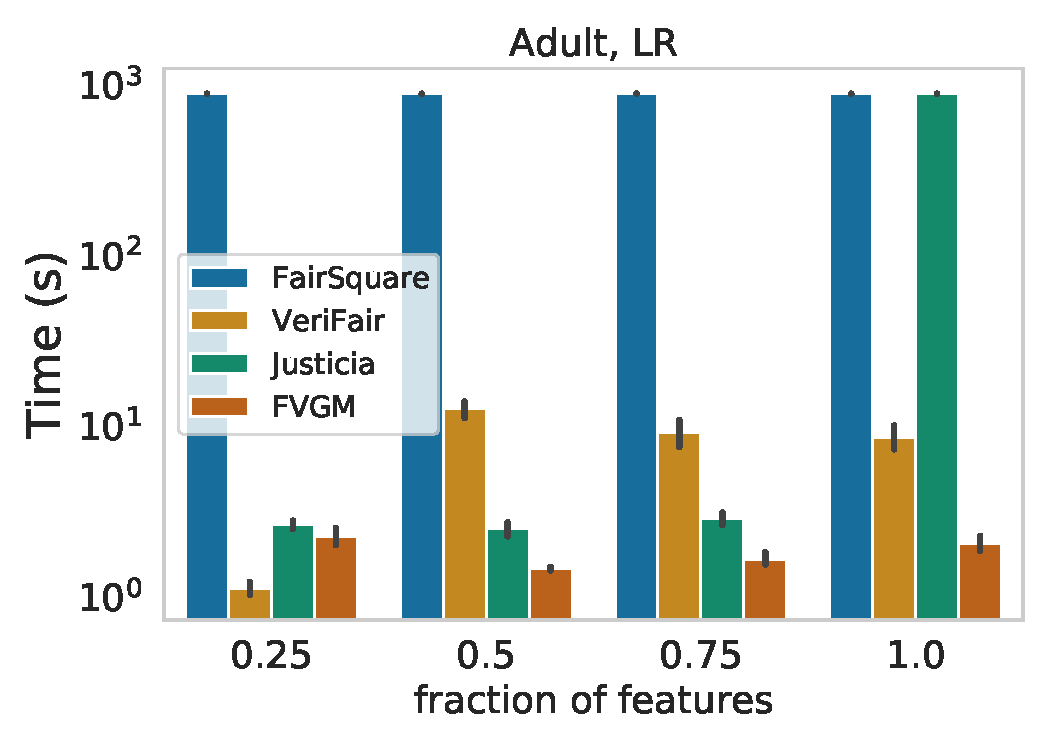
\includegraphics[scale=0.24]{figures/time_vary_features_Adult_LR}}
			\subfloat{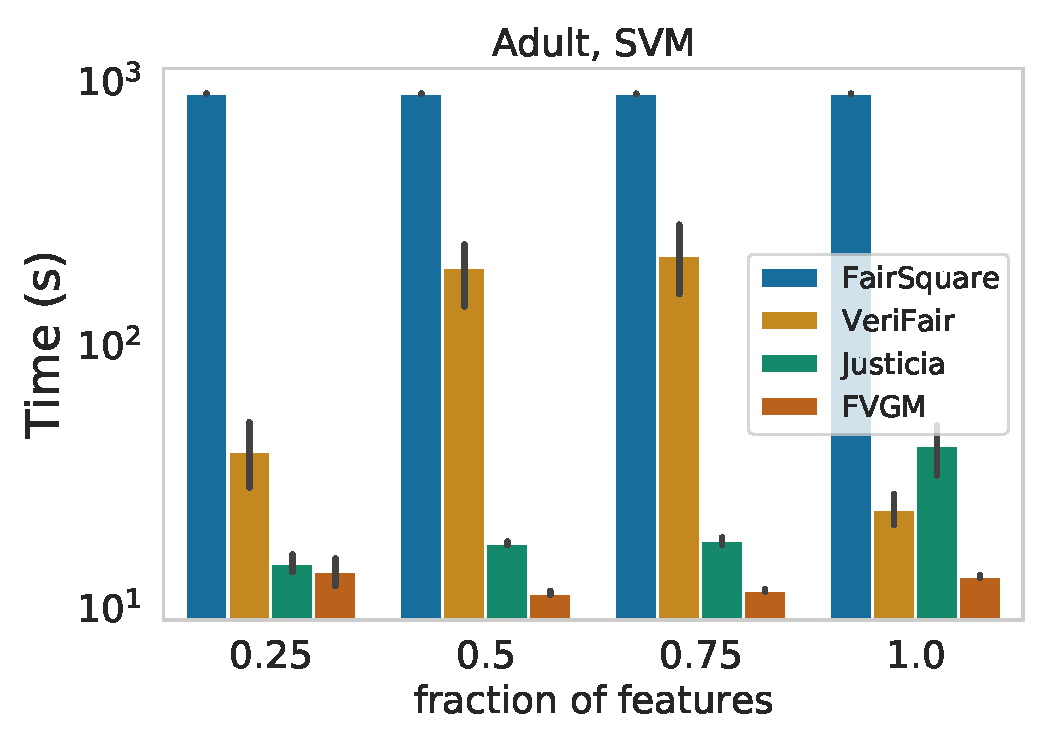
\includegraphics[scale=0.24]{figures/time_vary_features_Adult_SVM}}	\\		
			\subfloat{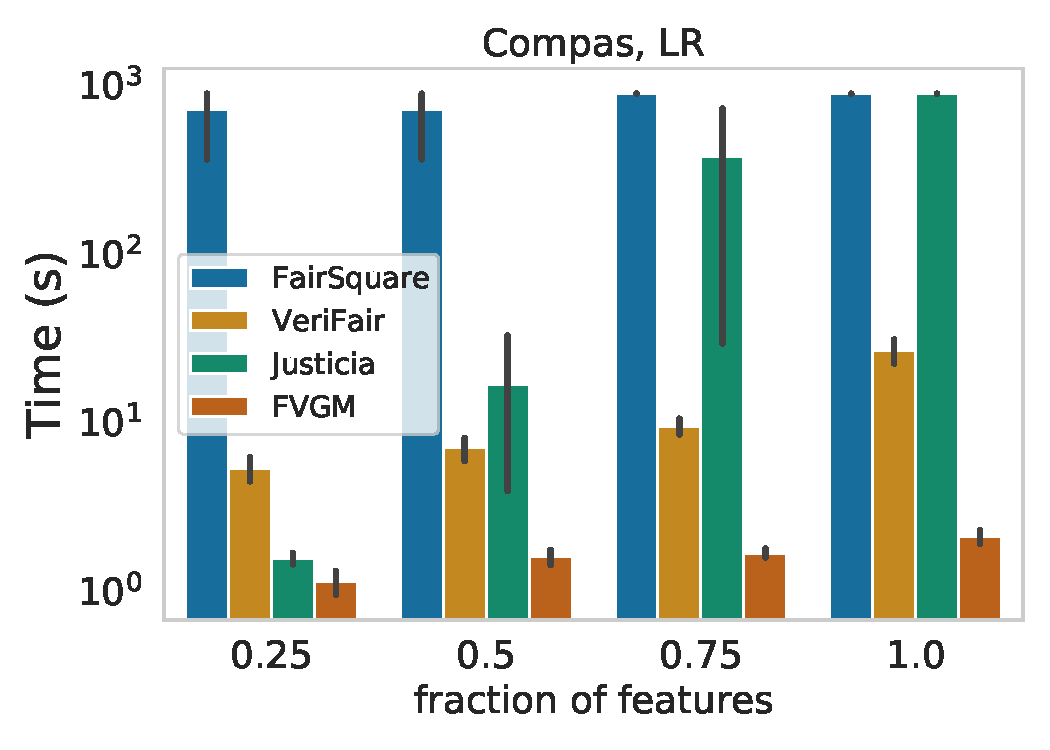
\includegraphics[scale=0.24]{figures/time_vary_features_Compas_LR}}
			\subfloat{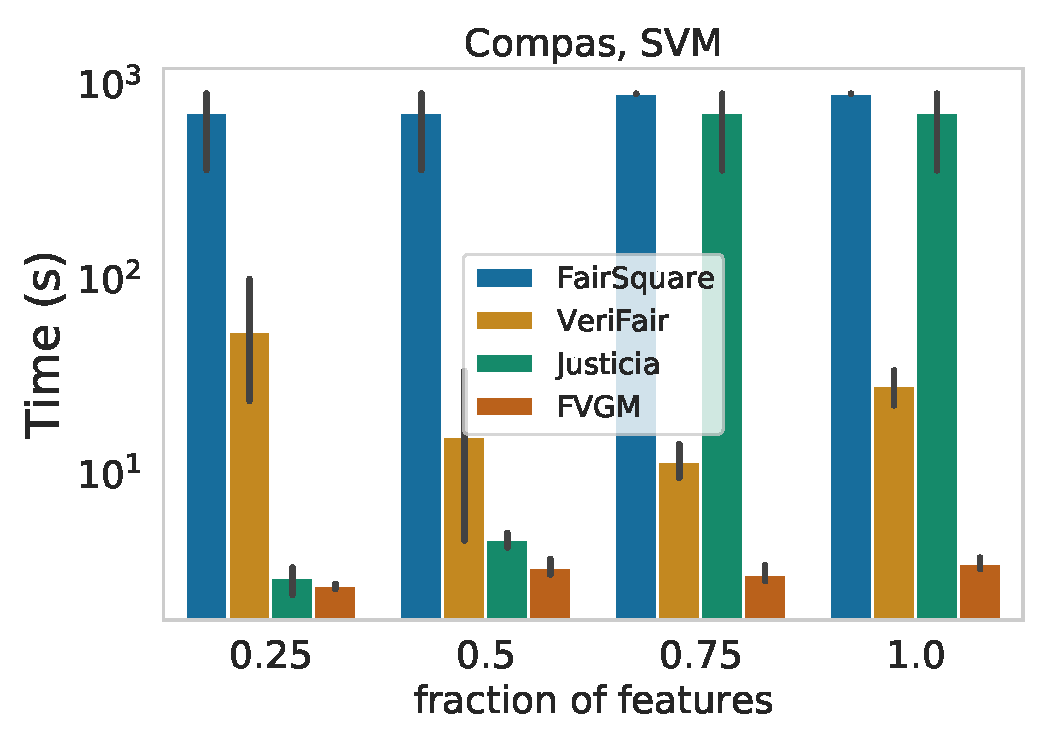
\includegraphics[scale=0.24]{figures/time_vary_features_Compas_SVM}}\\
			
			\subfloat{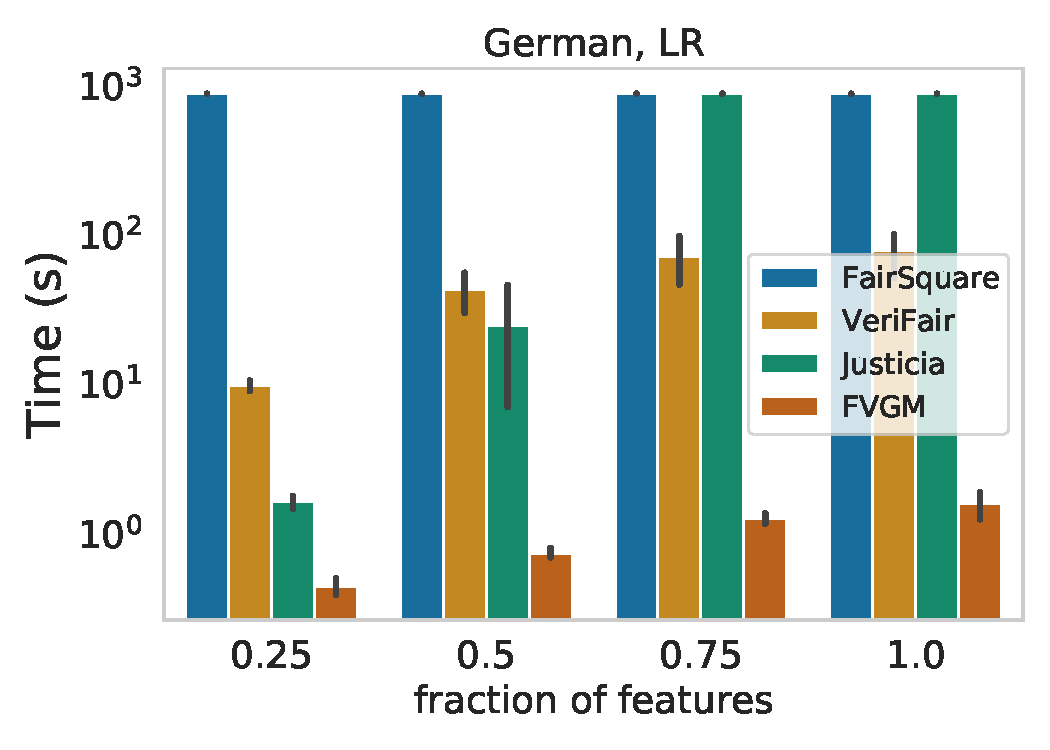
\includegraphics[scale=0.24]{figures/time_vary_features_German_LR}}
			\subfloat{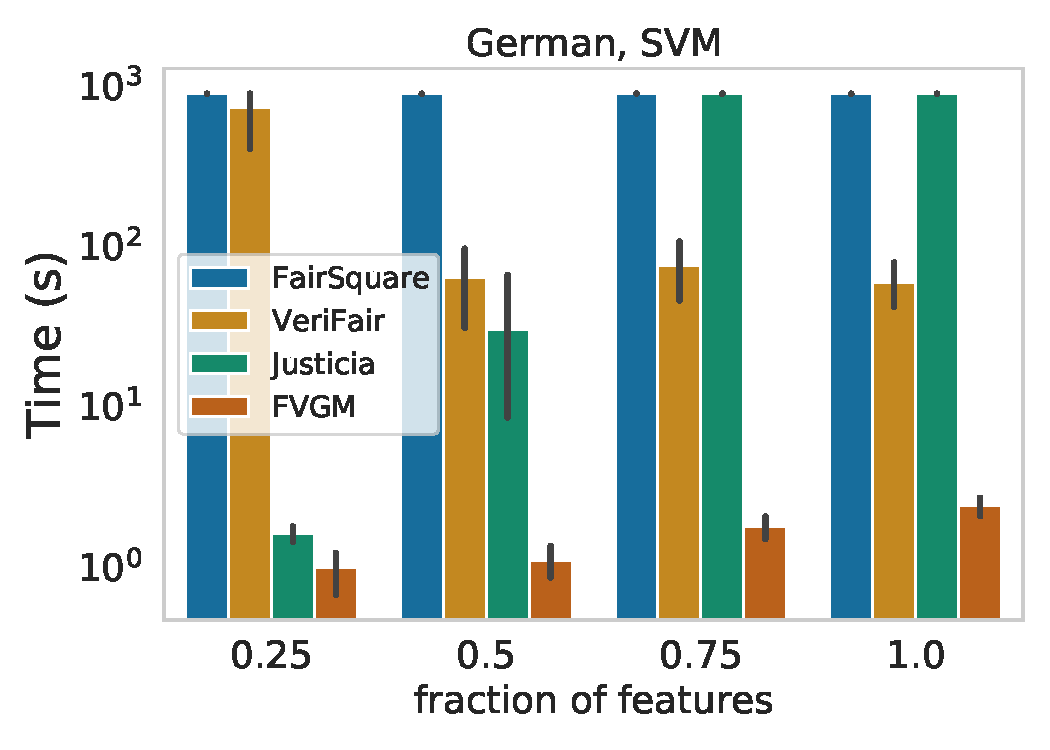
\includegraphics[scale=0.24]{figures/time_vary_features_German_SVM}}		\\
			\subfloat{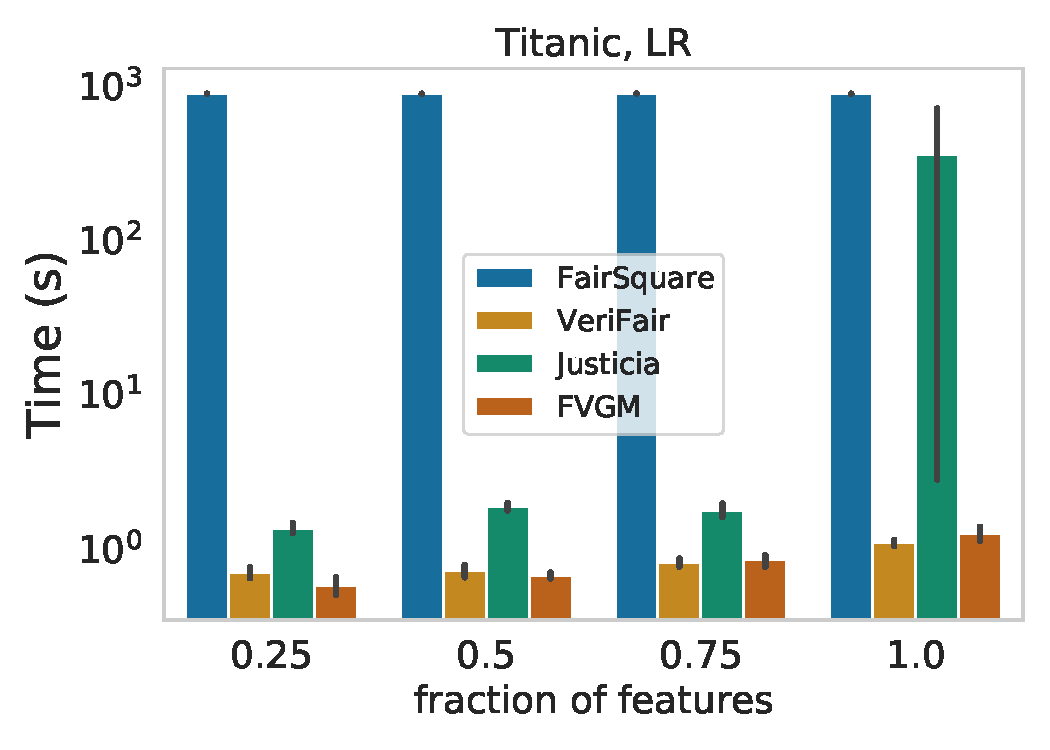
\includegraphics[scale=0.24]{figures/time_vary_features_Titanic_LR}}
			\subfloat{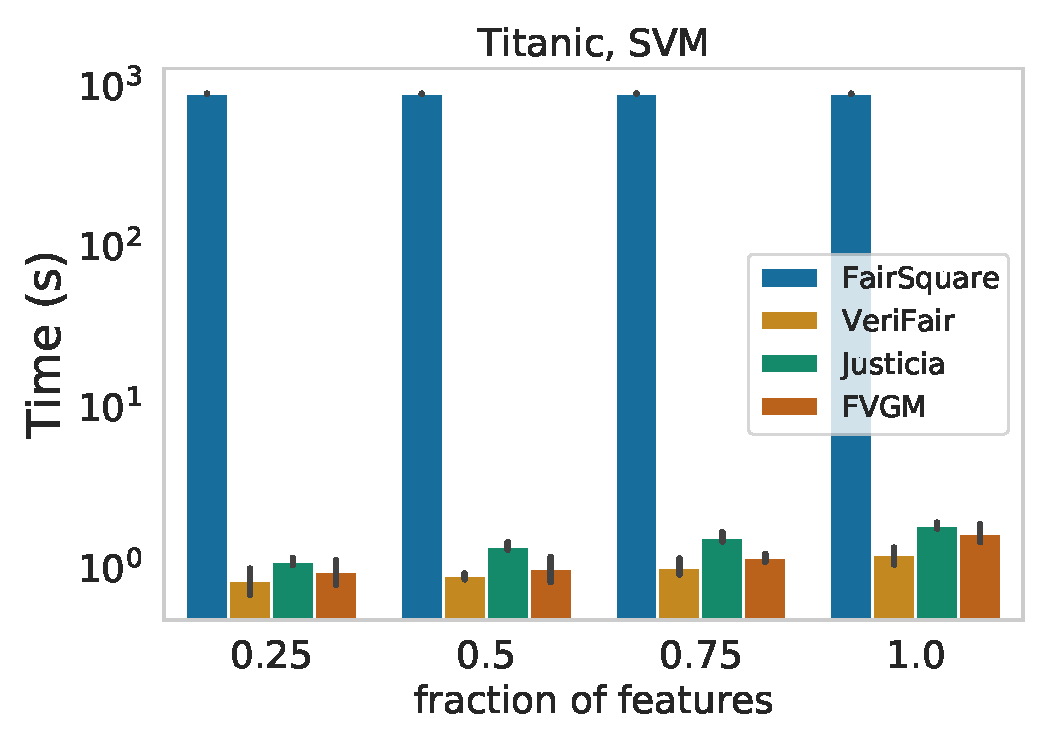
\includegraphics[scale=0.24]{figures/time_vary_features_Titanic_SVM}}\\
			
			\subfloat{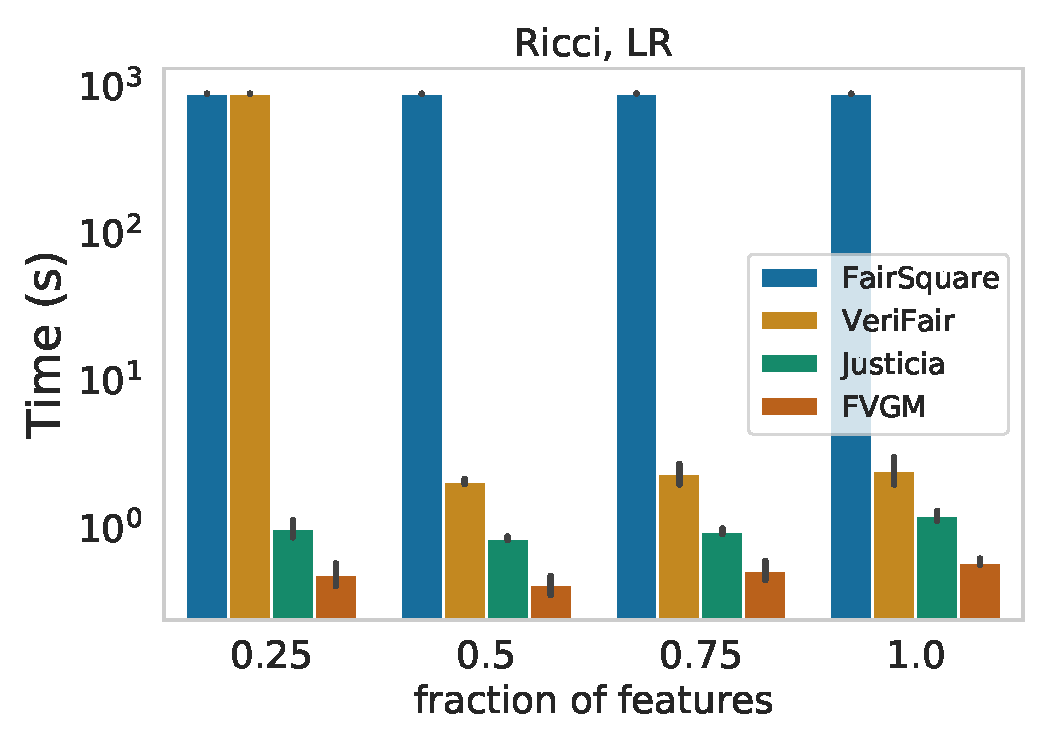
\includegraphics[scale=0.24]{figures/time_vary_features_Ricci_LR}}
			\subfloat{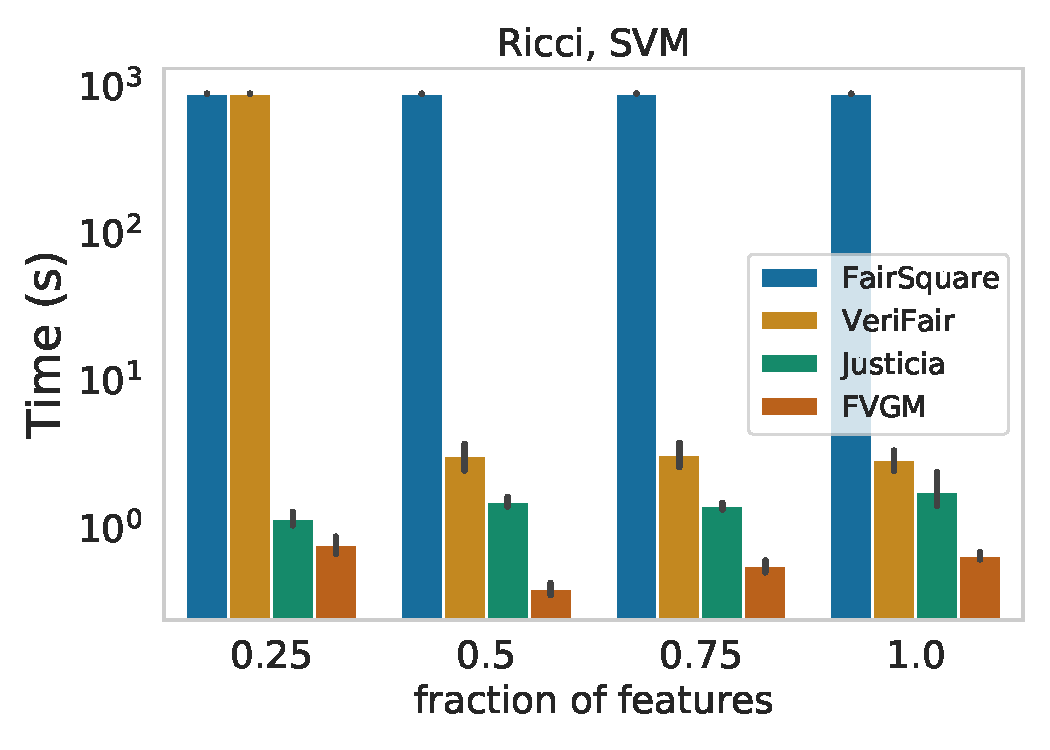
\includegraphics[scale=0.24]{figures/time_vary_features_Ricci_SVM}}
			
			\caption{Effect of number of features on the runtime of different datasets for LR and SVM classifiers.}
			\label{fig:time_vary_features}
			
			
			
		\end{center}
		
		
	\end{figure}
	
	
	\subsection{Scalability Comparison Among Different Verifiers}
	
	In Figure~\ref{fig:time_vary_features}, we present the runtime of different fairness verifiers while varying the number of features in different datasets. We observe that with an increase of features, the runtime increases in general.
	
	
	
	
	
	
	
	
	\begin{figure}
	\begin{center}
		\subfloat{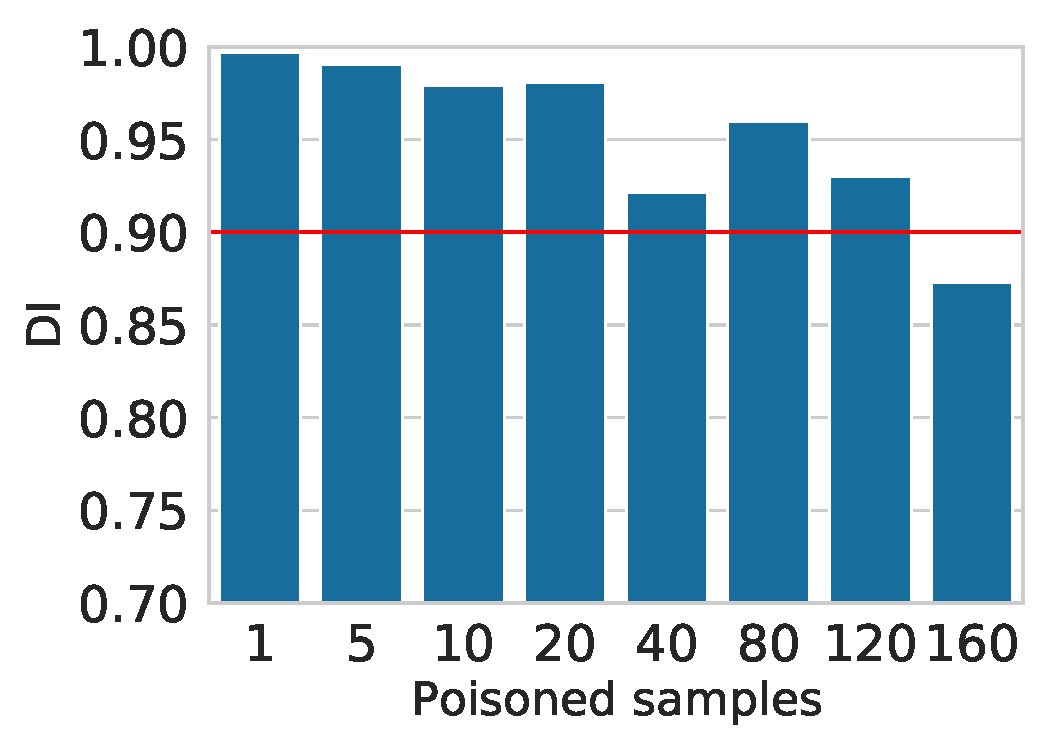
\includegraphics[scale=0.35]{figures/fairness/fvgm/disp_fairness_attack}}
		\subfloat{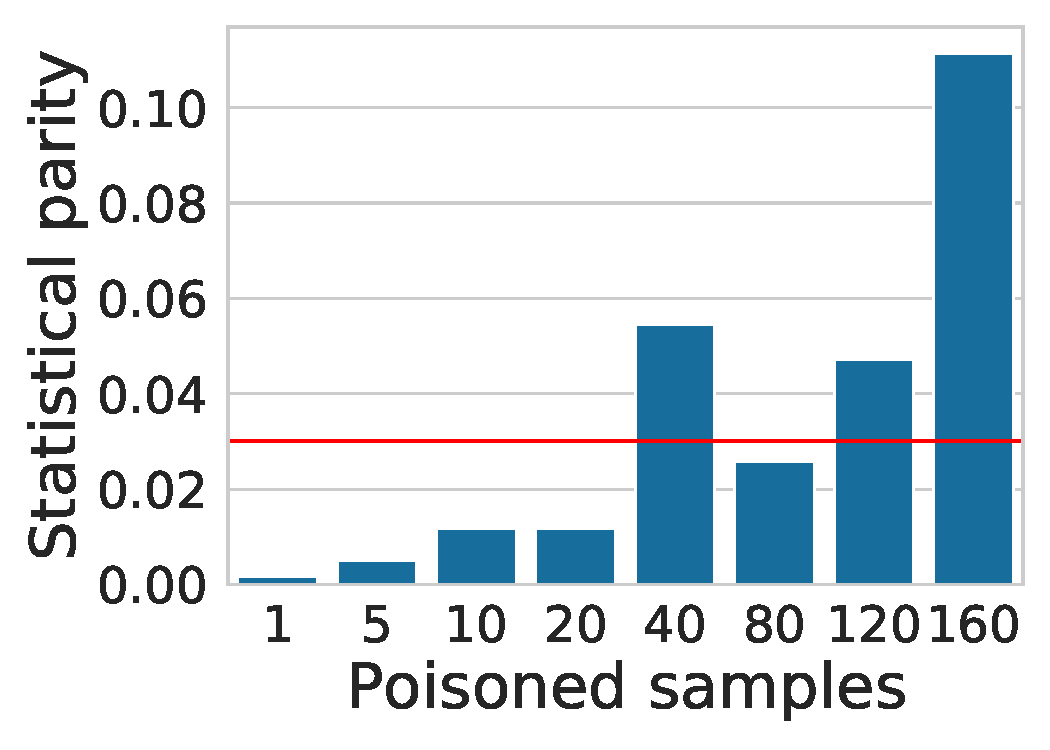
\includegraphics[scale=0.35]{figures/fairness/fvgm/stat_fairness_attack}}\\
	\end{center}
	\caption[Verifying fairness poisoning attack using {\fvgm}]{Verifying fairness poisoning attack using {\fvgm}. The red line denotes safety margin, which being exceeded denotes system-vulnerability by the attack algorithm. As the number of poisoned samples increase, disparate impact (DI) decreases and statistical parity (SP)  increases.}
	\label{fairness_fvgm_fig:attack_extended}
\end{figure}

	%\clearpage

\begin{table}[t!]
    \centering
        \setlength{\tabcolsep}{.3em}
%        \vspace*{-.3em}
            \begin{tabular}{lrrrrrrrrrrrrrrr}
                \toprule
                Dataset   & \multicolumn{3}{c}{Ricci} & \multicolumn{3}{c}{Titanic} & \multicolumn{3}{c}{COMPAS} &  \multicolumn{3}{c}{Adult} &
                \multicolumn{3}{c}{German} \\ 
                
                \cmidrule(lll){2-4}
                \cmidrule(lr){5-7}
                \cmidrule(lr){8-10}
                \cmidrule(lr){11-13}
                \cmidrule(lr){14-16}
                

                Classifier & 
                LR & SVC & DT &
                LR & SVC & DT &
                LR & SVC & DT &
                LR & SVC & DT &
                LR & SVC & DT \\
				 \midrule

{\framework} &  $ \textbf{0.1} $  &  $ \textbf{0.1} $  &  $ \textbf{0.1} $  &  $ \textbf{0.1} $  &  $ \textbf{0.1} $  &  $ 1.6 $  &  $ \textbf{0.4} $  &  $ \textbf{0.5} $  &  $ 121.7 $  &  $ \textbf{0.9} $  &  $ 1.8 $  &  $ \textbf{0.3} $  &  $ \textbf{1.4} $  &  $ \textbf{1.4} $  &  $ 2.3 $  \\ 
Justicia &  $ 2.2 $  &  $ 2.2 $  &  $ \textbf{0.1} $  &  $ 0.3 $  &  $ 0.2 $  &  $ \textbf{0.3} $  & \textemdash & \textemdash &  $ \textbf{0.3} $  & \textemdash &  $ \textbf{1.7} $  &  $ 0.4 $  & \textemdash & \textemdash &  $ \textbf{0.2} $  \\ 
VeriFair &  $ 2.0 $  &  $ 1.8 $  &  $ 1.9 $  &  $ 0.5 $  &  $ 0.4 $  &  $ 17.2 $  &  $ 12.2 $  &  $ 11.6 $  &  $ 377.1 $  &  $ 7.3 $  &  $ 21.7 $  &  $ 57.9 $  &  $ 19.2 $  &  $ 28.8 $  &  $ 78.5 $  \\ 
FairSquare & \textemdash & \textemdash &  $ 4.6 $  & \textemdash & \textemdash &  $ 432.9 $  & \textemdash & \textemdash & \textemdash & \textemdash & \textemdash & \textemdash & \textemdash & \textemdash & \textemdash \\ 



















	
		
			
				
				
				
				
				
				
				


    \end{tabular}
\caption{Scalability of different verifiers in terms of execution time (in seconds).  DT and LR refer to decision tree and logistic regression respectively. `\textemdash'~ refers to timeout. \red{Restricted experiments with Boolean single sensitive attribute.}}
\label{tab:FS_VF_Justicia}
%\vspace*{-1em}
\end{table}








\begin{table}[t!]
	\centering
	\setlength{\tabcolsep}{.3em}
	%        \vspace*{-.3em}
	\begin{tabular}{lrrrrrrrrrrrrrrr}
		\toprule
		Dataset   & \multicolumn{3}{c}{Ricci} & \multicolumn{3}{c}{Titanic} & \multicolumn{3}{c}{COMPAS} &  \multicolumn{3}{c}{Adult} &
		\multicolumn{3}{c}{German} \\ 
		
		\cmidrule(lr){2-4}
		\cmidrule(lr){5-7}
		\cmidrule(lr){8-10}
		\cmidrule(lr){11-13}
		
		
		Classifier & 
		LR & SVC & DT &
		LR & SVC & DT &
		LR & SVC & DT &
		LR & SVC & DT &
		LR & SVC & DT \\
		\midrule
		
		{\framework} &  $ 0.86 $  &  $ 1.0 $  &  $ 1.0 $  &  $ 0.16 $  &  $ 0.0 $  &  $ 0.59 $  &  $ 0.74 $  &  $ 0.85 $  &  $ 0.94 $  &  $ 0.65 $  &  $ 1.0 $  &  $ 0.49 $  &  $ 0.82 $  &  $ 0.9 $  &  $ 0.94 $  \\ 
		Justicia &  $ 0.26 $  &  $ 0.36 $  &  $ 0.3 $  &  $ 0.14 $  &  $ 0.0 $  &  $ 0.55 $  & \textemdash & \textemdash &  $ 0.79 $  & \textemdash &  $ 0.85 $  &  $ 0.22 $  & \textemdash & \textemdash &  $ 0.89 $  \\ 
		VeriFair &  $ 0.28 $  &  $ 0.4 $  &  $ 0.49 $  &  $ 0.1 $  &  $ 0.0 $  &  $ 0.87 $  &  $ 0.79 $  &  $ 0.74 $  &  $ 0.97 $  &  $ 0.79 $  &  $ 0.88 $  &  $ 0.93 $  &  $ 0.66 $  &  $ 0.64 $  &  $ 0.89 $  \\ 
		FairSquare & \textemdash & \textemdash &  $ 0.52 $  & \textemdash & \textemdash &  $ 0.87 $  & \textemdash & \textemdash & \textemdash & \textemdash & \textemdash & \textemdash & \textemdash & \textemdash & \textemdash \\ 
		
		
		
		
		
		
		
		
		
		
		
		
		
		
		
	\end{tabular}
	\caption{Computed disparate impact by different fairness verifiers on different datasets and classifiers.  DT and LR refer to decision tree and logistic regression respectively. `\textemdash'~ refers to timeout.}
	\label{tab:FS_VF_Justicia}
	%\vspace*{-1em}
\end{table}
	%
\begin{figure}
		\begin{center}
			\subfloat[]{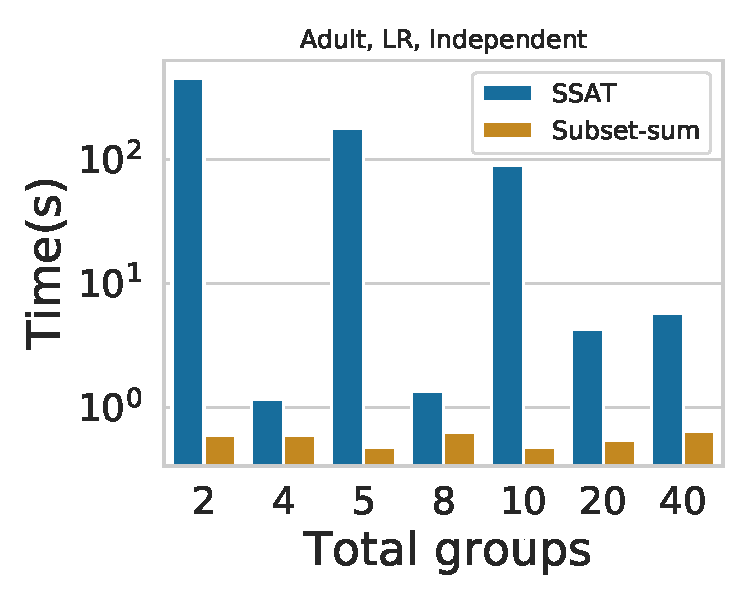
\includegraphics[scale=0.25]{figures/ssat_vs_subsetsum_Independent_Adult_LR}}
			\subfloat[]{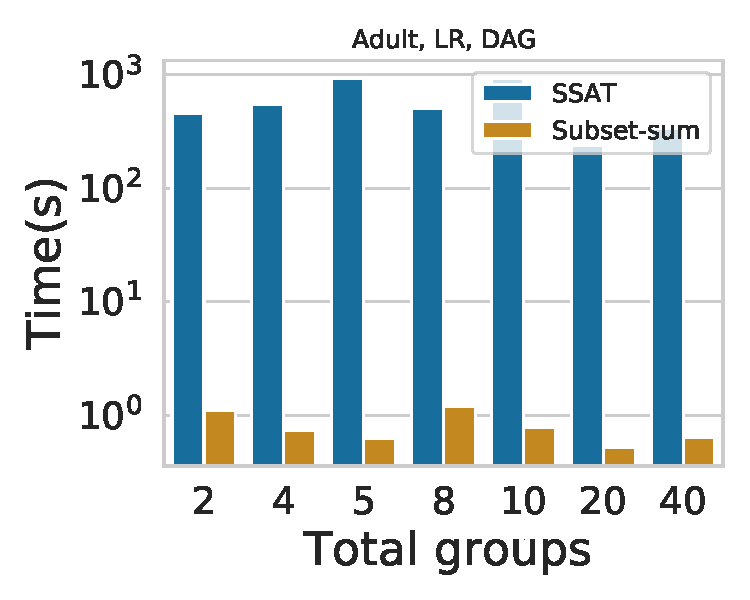
\includegraphics[scale=0.25]{figures/ssat_vs_subsetsum_DAG_Adult_LR}}
			\subfloat[]{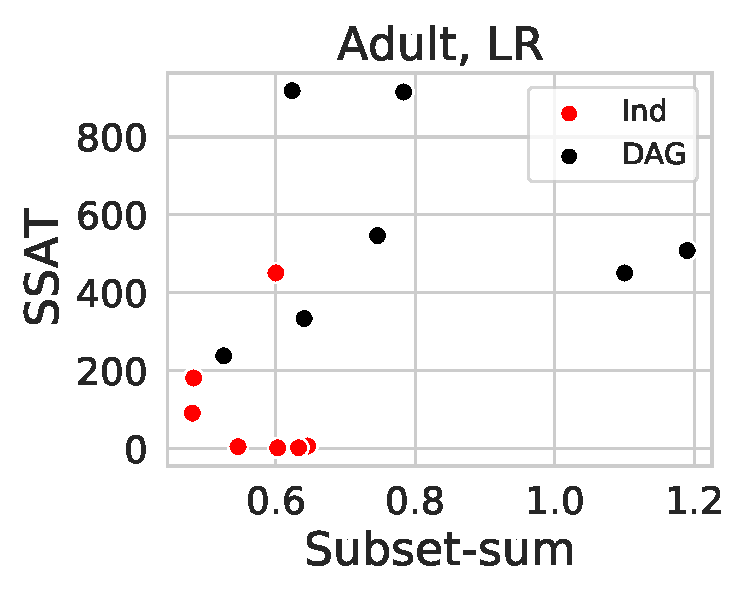
\includegraphics[scale=0.25]{figures/ssat_vs_subsetsum_time_scatter_plot_Adult_LR}}\\
			
			\subfloat[]{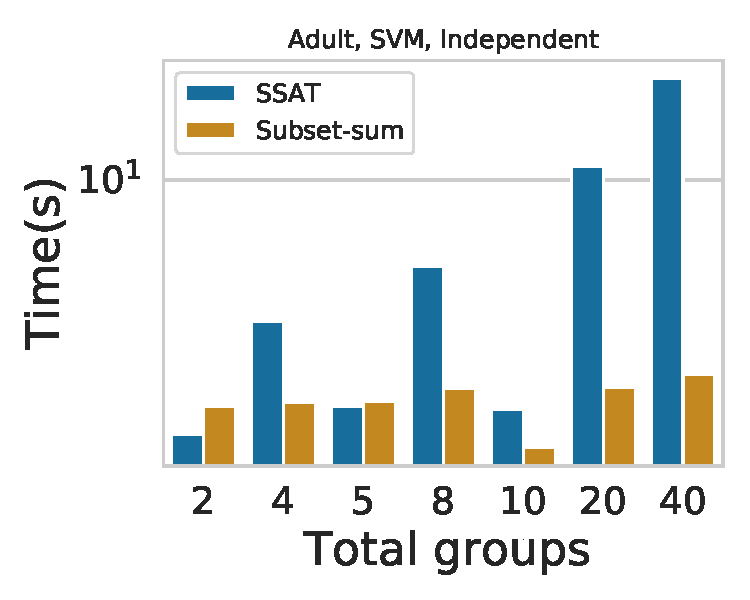
\includegraphics[scale=0.25]{figures/ssat_vs_subsetsum_Independent_Adult_SVM}}
			\subfloat[]{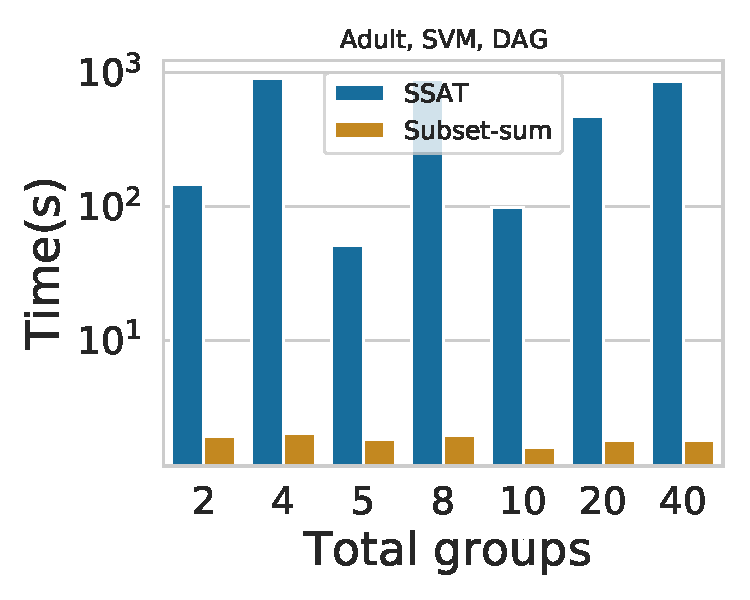
\includegraphics[scale=0.25]{figures/ssat_vs_subsetsum_DAG_Adult_SVM}}
			\subfloat[]{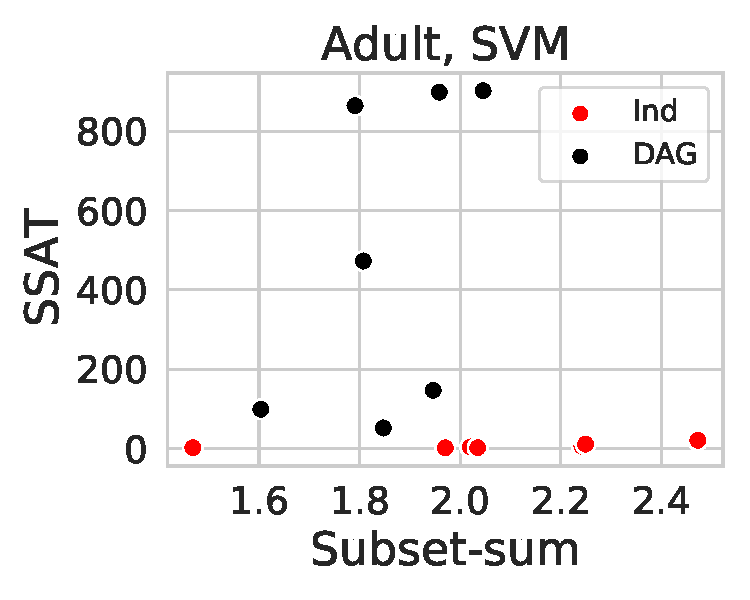
\includegraphics[scale=0.25]{figures/ssat_vs_subsetsum_time_scatter_plot_Adult_SVM}}\\
			
			
			\subfloat[]{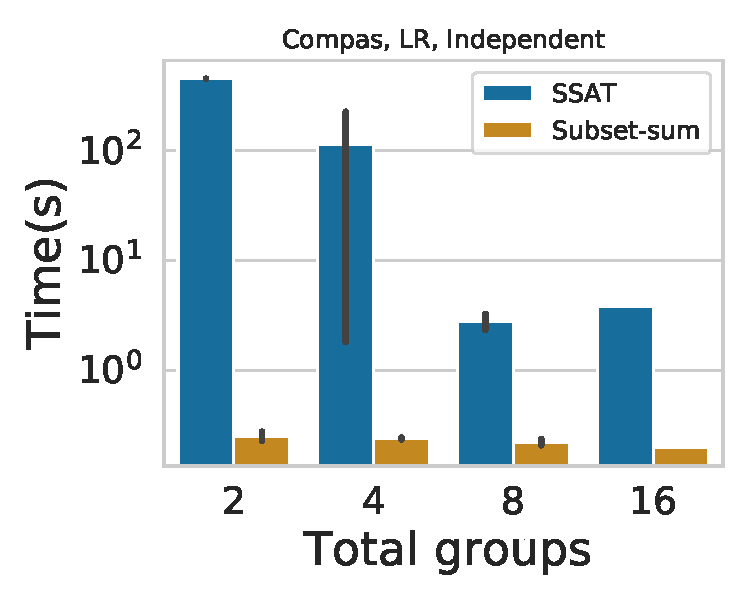
\includegraphics[scale=0.25]{figures/ssat_vs_subsetsum_Independent_Compas_LR}}
			\subfloat[]{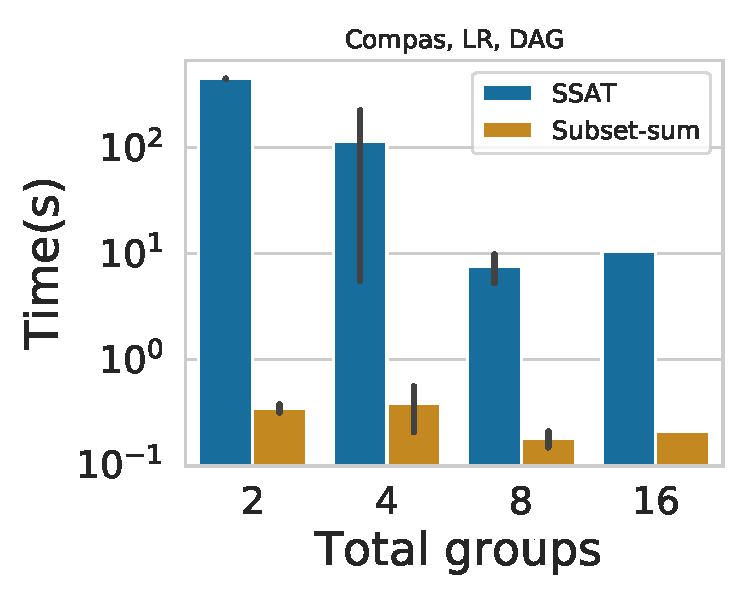
\includegraphics[scale=0.25]{figures/ssat_vs_subsetsum_DAG_Compas_LR}}
			\subfloat[]{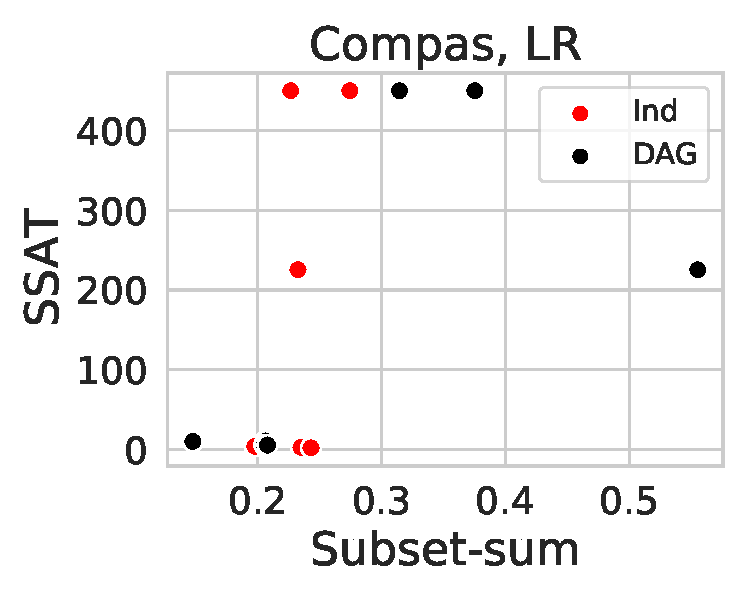
\includegraphics[scale=0.25]{figures/ssat_vs_subsetsum_time_scatter_plot_Compas_LR}}\\
			
			\subfloat[]{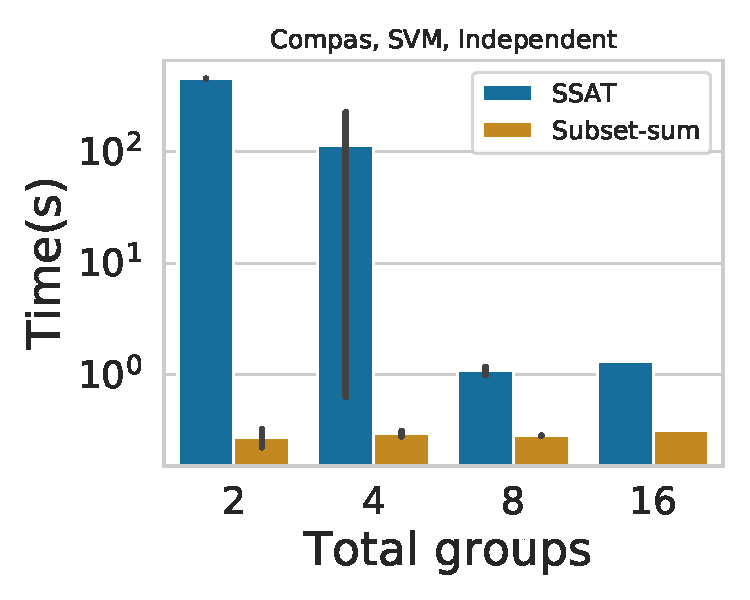
\includegraphics[scale=0.25]{figures/ssat_vs_subsetsum_Independent_Compas_SVM}}
			\subfloat[]{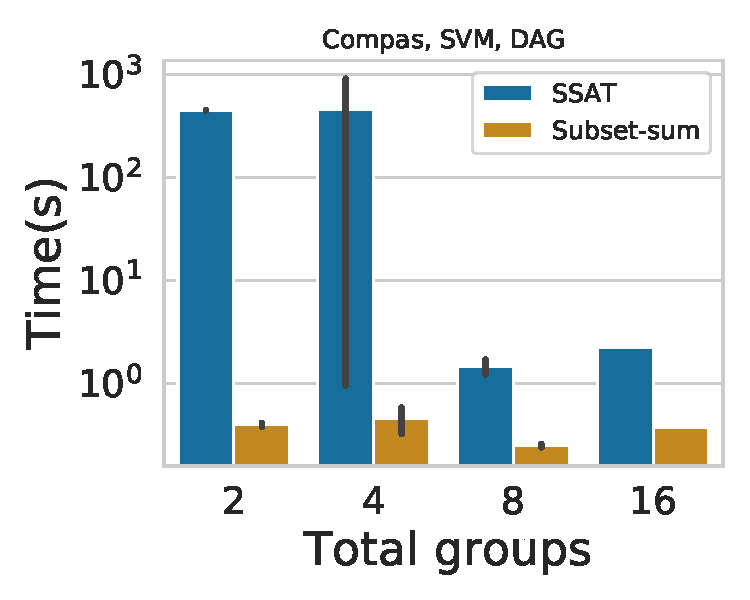
\includegraphics[scale=0.25]{figures/ssat_vs_subsetsum_DAG_Compas_SVM}}
			\subfloat[]{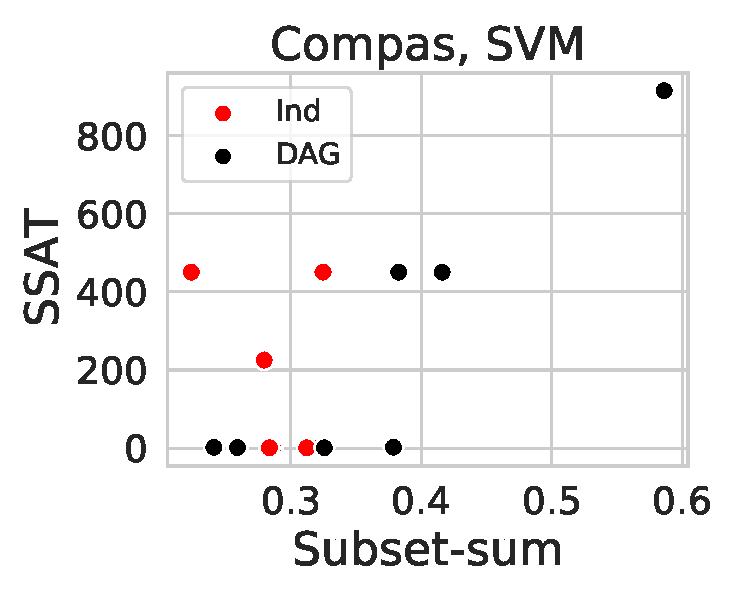
\includegraphics[scale=0.25]{figures/ssat_vs_subsetsum_time_scatter_plot_Compas_SVM}}\\
			
			\subfloat[]{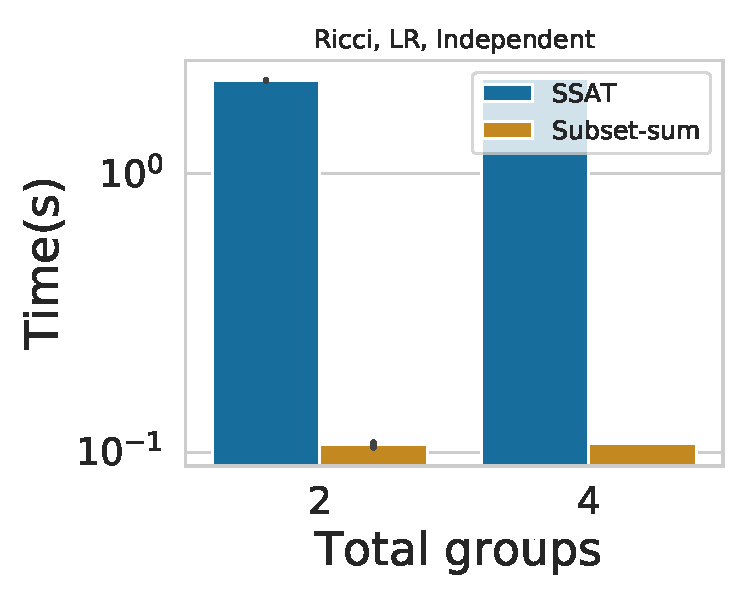
\includegraphics[scale=0.25]{figures/ssat_vs_subsetsum_Independent_Ricci_LR}}
			\subfloat[]{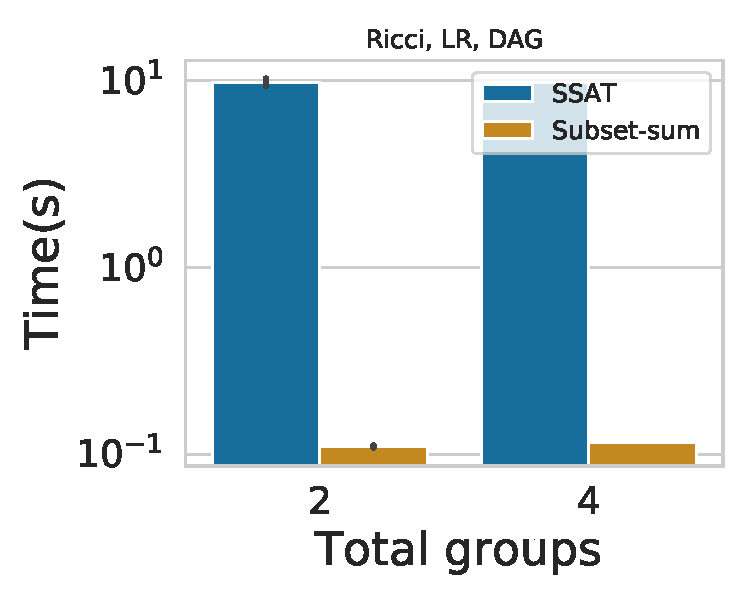
\includegraphics[scale=0.25]{figures/ssat_vs_subsetsum_DAG_Ricci_LR}}
			\subfloat[]{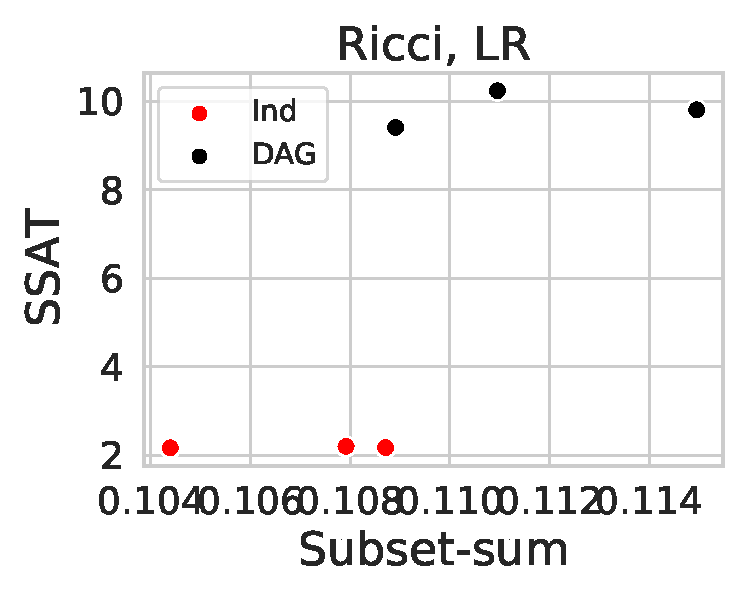
\includegraphics[scale=0.25]{figures/ssat_vs_subsetsum_time_scatter_plot_Ricci_LR}}\\
			
			\subfloat[]{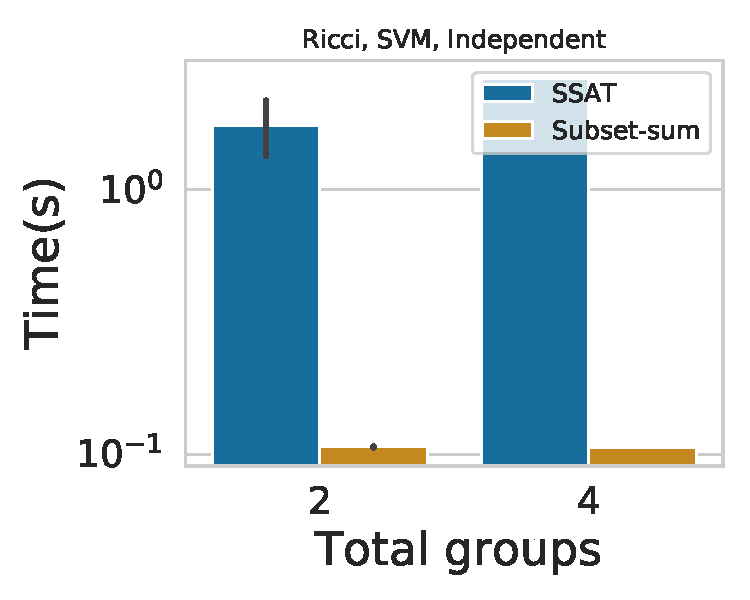
\includegraphics[scale=0.25]{figures/ssat_vs_subsetsum_Independent_Ricci_SVM}}
			\subfloat[]{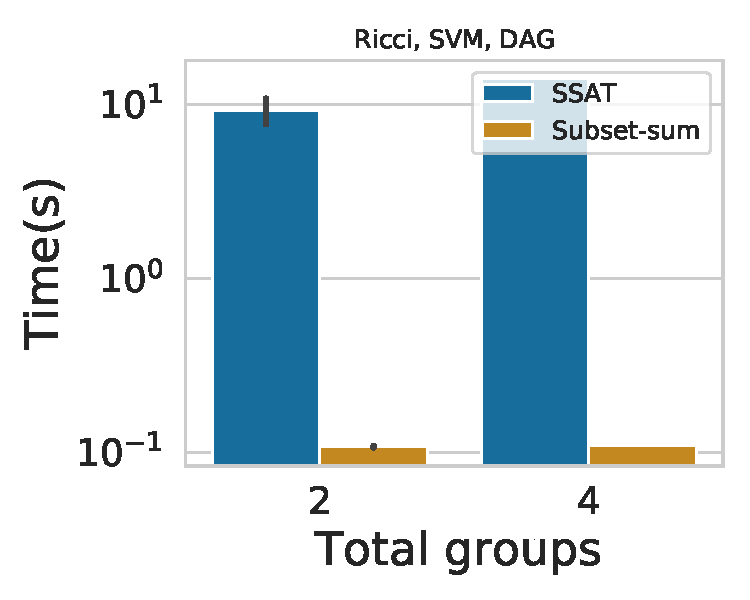
\includegraphics[scale=0.25]{figures/ssat_vs_subsetsum_DAG_Ricci_SVM}}
			\subfloat[]{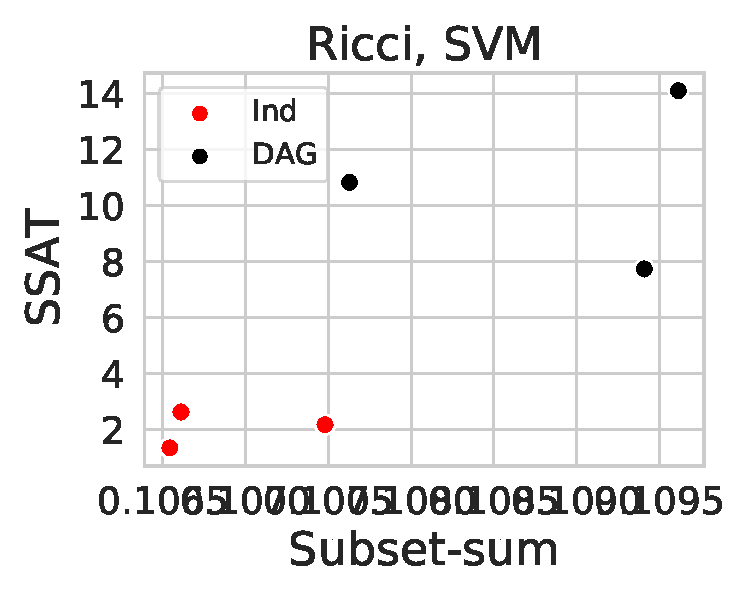
\includegraphics[scale=0.25]{figures/ssat_vs_subsetsum_time_scatter_plot_Ricci_SVM}}\\
			
			
			\subfloat[]{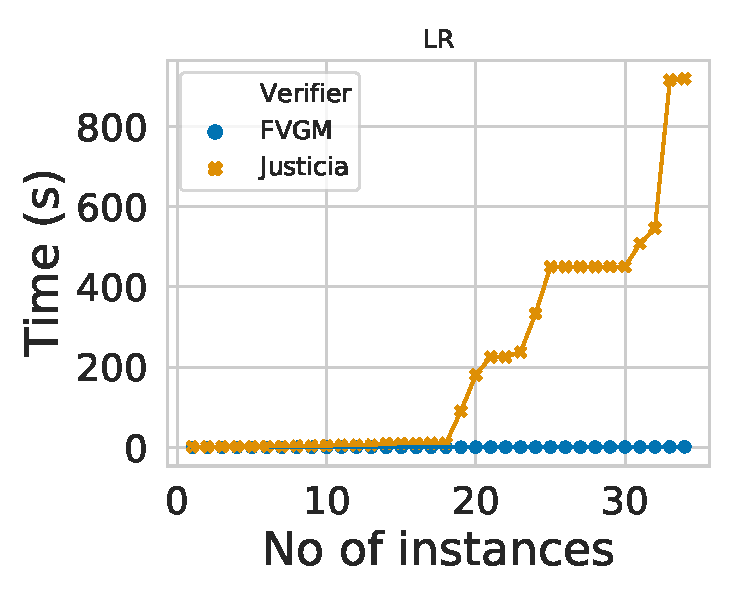
\includegraphics[scale=0.25]{figures/cactus_subsetsum_ssat_LR_time_.pdf}}
			\subfloat[]{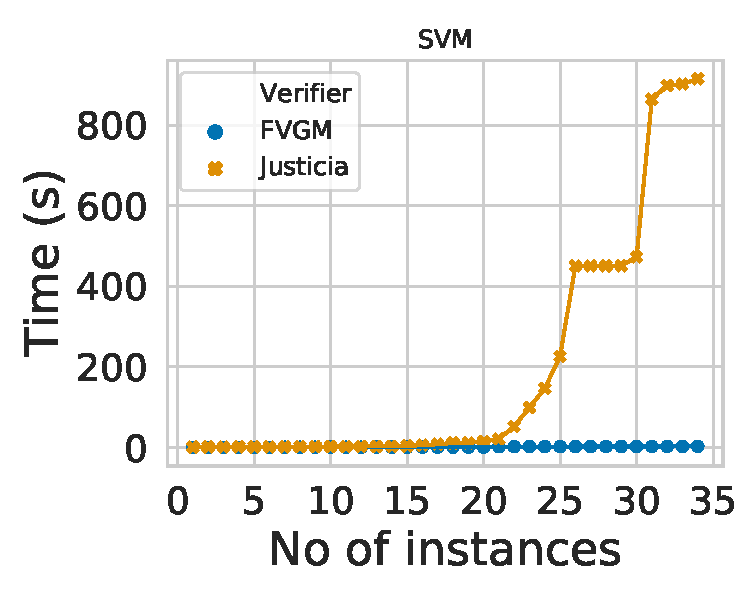
\includegraphics[scale=0.25]{figures/cactus_subsetsum_ssat_SVM_time_.pdf}}
			

		\end{center}
		
		\caption{Scalability between {\framework} and Justicia. \red{Each instance represents the runtime of verifying on a dataset and a set of sensitive attributes.}}
\end{figure}
	
	
	

	%
\begin{table*}       
    \centering
        \setlength{\tabcolsep}{.2em}
            \begin{tabular}{ll
            				ccc
            				ccc
            				ccc
            				ccc
            				ccc
            				ccc}
                \toprule
                \multirow{3}{*}{Encoding}& Dataset $ \rightarrow $   & 
                \multicolumn{8}{c}{Adult} &
%                \multicolumn{6}{c}{German} &
                \multicolumn{8}{c}{COMPAS} \\ 
                \cmidrule(lr){3-10}
                \cmidrule(lr){11-18}
                & Protected  $ \rightarrow $ & 
                \multicolumn{4}{c}{Race}   & \multicolumn{4}{c}{Sex}  &
%                \multicolumn{3}{c}{Age}   & \multicolumn{3}{c}{Sex}  &
                \multicolumn{4}{c}{Race}   & \multicolumn{4}{c}{Sex}
                \\ 
                \cmidrule(lr){3-6}
                \cmidrule(lr){7-10}
                \cmidrule(lr){11-14}
                \cmidrule(lr){15-18}

                 & Algorithm  $ \rightarrow $ &  
                orig. & RCO &
                orig. & CPP &
                orig. & RCO &
                orig. & CPP &
                orig. & RCO &
                orig. & CPP &
				orig. & RCO &
				orig. & CPP &
               \\
                \midrule
          
              
              
			Ind
			& DI&  $ 0.76 $ &  $ 0.67 $ &  $ 1.00 $ &  $ 0.71 $ &  $ 0.30 $ &  $ \mathbf{0.63} $ &  $ 1.00 $ &  $ 0.06 $ &  $ 0.96 $ &  $ 0.62 $ &  $ 1.00 $ &  $ \mathbf{1.00} $ &  $ 0.60 $ &  $ 0.55 $ &  $ 0.80 $ &  $ 0.75 $  \\
			& SP&  $ 0.15 $ &  $ 0.16 $ &  $ 0.00 $ &  $ 0.05 $ &  $ 0.53 $ &  $ \mathbf{0.21} $ &  $ 0.00 $ &  $ 0.13 $ &  $ 0.01 $ &  $ 0.14 $ &  $ 0.00 $ &  $ \mathbf{0.00} $ &  $ 0.13 $ &  $ \mathbf{0.13} $ &  $ 0.11 $ &  $ \mathbf{0.10} $  \\
			\midrule
			DAG
			& DI&  $ 0.73 $ &  $ 0.68 $ &  $ 1.00 $ &  $ 0.71 $ &  $ 0.33 $ &  $ \mathbf{0.68} $ &  $ 1.00 $ &  $ 0.05 $ &  $ 0.93 $ &  $ 0.62 $ &  $ 1.00 $ &  $ \mathbf{1.00} $ &  $ 0.62 $ &  $ 0.56 $ &  $ 0.80 $ &  $ 0.75 $  \\
			& SP&  $ 0.17 $ &  $ \mathbf{0.15} $ &  $ 0.00 $ &  $ 0.05 $ &  $ 0.51 $ &  $ \mathbf{0.17} $ &  $ 0.00 $ &  $ 0.15 $ &  $ 0.02 $ &  $ 0.14 $ &  $ 0.00 $ &  $ \mathbf{0.00} $ &  $ 0.13 $ &  $ \mathbf{0.13} $ &  $ 0.11 $ &  $ \mathbf{0.10} $  \\
			
			
               
            \bottomrule
    \end{tabular}
\caption{Logistic regression and two encodings: learn and learn-dependency. ``\textemdash'' refers to timeout of DAG learner (Notears). }
\end{table*}



\begin{table*}       
	\centering
	        \setlength{\tabcolsep}{.2em}
	\begin{tabular}{ll
			ccc
			ccc
			%            				ccc
			%            				ccc
			ccc
			ccc}
		\toprule
		\multirow{3}{*}{Classifier}& Dataset $ \rightarrow $   & 
		\multicolumn{6}{c}{Adult} &
		%                \multicolumn{6}{c}{German} &
		\multicolumn{6}{c}{COMPAS} \\ 
		\cmidrule(lr){3-8}
		\cmidrule(lr){9-14}
		%                \cmidrule(lr){15-20}
		& Protected  $ \rightarrow $ & 
		\multicolumn{3}{c}{Race}   & \multicolumn{3}{c}{Sex}  &
		%                \multicolumn{3}{c}{Age}   & \multicolumn{3}{c}{Sex}  &
		\multicolumn{3}{c}{Race}   & \multicolumn{3}{c}{Sex}
		\\ 
		\cmidrule(lr){3-5}
		\cmidrule(lr){6-8}
		\cmidrule(lr){9-11}
		\cmidrule(lr){12-14}
		%                \cmidrule(lr){15-17}
		%                \cmidrule(lr){18-20}
		
		& Algorithm  $ \rightarrow $ &  
		orig. & RW & OP & 
		orig. & RW & OP &
		%                orig. & RW & OP &
		%                orig. & RW & OP &
		orig. & RW & OP &
		orig. & RW & OP \\ 
		\midrule
		
		
		
		\multirow{3}{*}{\shortstack{Logistic \\ regression}}
		& Disparte impact&  $ 0.41 $ &  $ \mathbf{0.67} $ &  $ \mathbf{0.97} $ &  $ 0.04 $ &  $ \mathbf{1.00} $ &  $ \mathbf{0.76} $ &  $ 0.78 $ &  $ 0.49 $ &  $ 0.63 $ &  $ 0.64 $ &  $ 0.63 $ &  $ \mathbf{1.00} $  \\
		& Stat. parity&  $ 0.07 $ &  $ \mathbf{0.05} $ &  $ \mathbf{0.00} $ &  $ 0.16 $ &  $ \mathbf{0.00} $ &  $ \mathbf{0.02} $ &  $ 0.09 $ &  $ 0.31 $ &  $ 0.21 $ &  $ 0.16 $ &  $ 0.21 $ &  $ \mathbf{0.00} $  \\
		& Equalized odds&  $ 0.03 $ &  $ \mathbf{0.02} $ &  $ \mathbf{0.00} $ &  $ 0.08 $ &  $ \mathbf{0.00} $ &  $ \mathbf{0.06} $ &  $ 0.09 $ &  $ 0.31 $ &  $ 0.20 $ &  $ 0.17 $ &  $ 0.20 $ &  $ \mathbf{0.00} $  \\
		\midrule
		\multirow{3}{*}{\shortstack{Decision \\ tree}}
		& Disparte impact&  $ 0.65 $ &  $ \mathbf{1.00} $ &  $ \mathbf{0.80} $ &  $ 0.00 $ &  $ \mathbf{1.00} $ &  $ \mathbf{0.92} $ &  $ 0.96 $ &  $ \mathbf{0.97} $ &  $ \mathbf{1.00} $ &  $ 0.82 $ &  $ \mathbf{1.00} $ &  $ \mathbf{0.95} $  \\
		& Stat. parity&  $ 0.04 $ &  $ \mathbf{0.00} $ &  $ \mathbf{0.03} $ &  $ 0.17 $ &  $ \mathbf{0.00} $ &  $ \mathbf{0.01} $ &  $ 0.02 $ &  $ \mathbf{0.01} $ &  $ \mathbf{0.00} $ &  $ 0.07 $ &  $ \mathbf{0.00} $ &  $ \mathbf{0.02} $  \\
		& Equalized odds&  $ 0.12 $ &  $ \mathbf{-0.00} $ &  $ \mathbf{0.03} $ &  $ 0.45 $ &  $ \mathbf{0.00} $ &  $ \mathbf{0.06} $ &  $ 0.02 $ &  $ \mathbf{0.01} $ &  $ \mathbf{0.00} $ &  $ 0.07 $ &  $ \mathbf{0.00} $ &  $ \mathbf{0.06} $  \\
		
		
		
		
		
		
		
		
		\bottomrule
	\end{tabular}
	\caption{Verification of different fairness enhancing algorithms for multiple datasets and classifiers using {\framework}. Numbers in bold refer to fairness improvement  compared against the unprocessed (orig.) dataset. RW and OP refer to reweighing and optimized-preprocessing algorithm respectively. }
\end{table*}
	\begin{figure}
	\begin{center}
		\subfloat{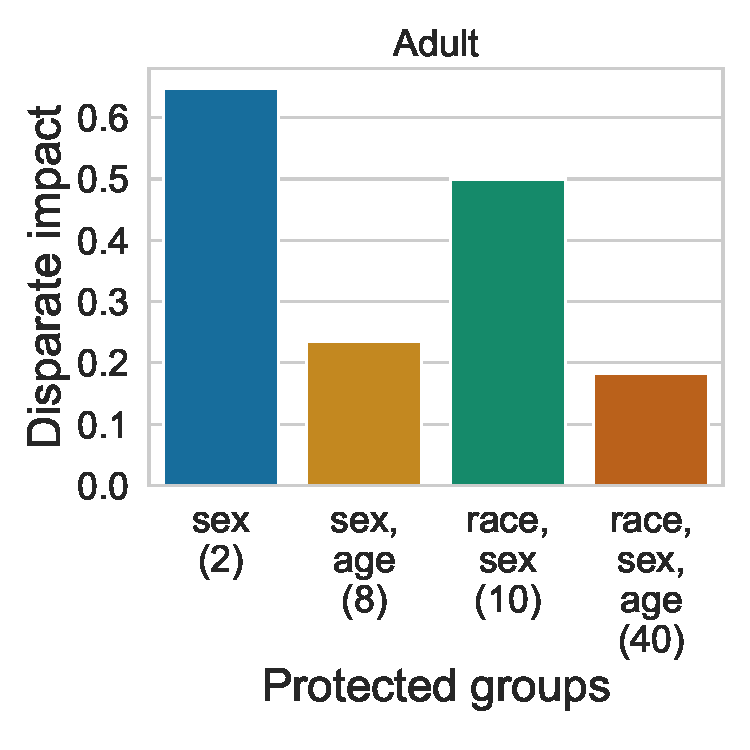
\includegraphics[scale=0.4]{figures/fairness/fvgm/sensitive_attribute__Disparate_impact_Adult_LR_Learn-efficient-dependency}}
		\subfloat{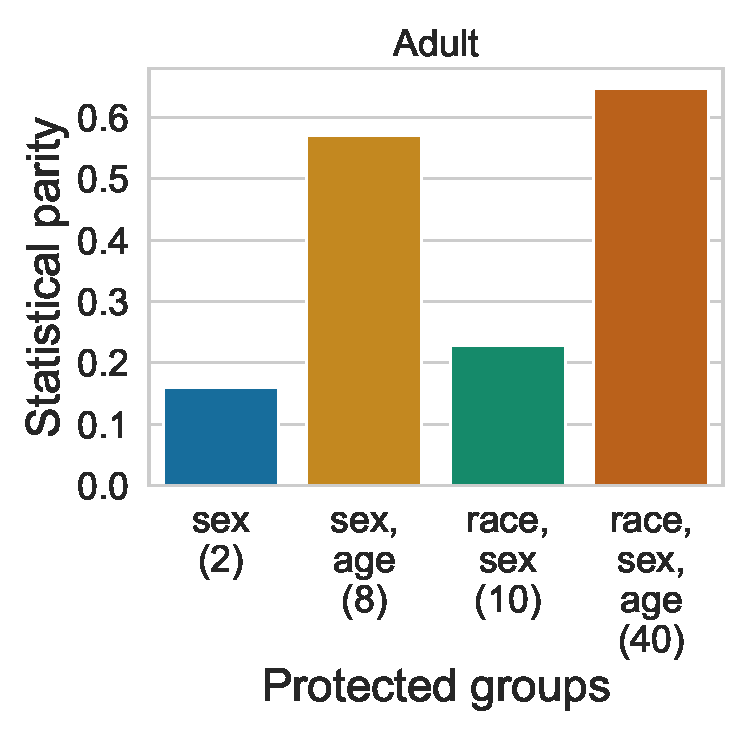
\includegraphics[scale=0.4]{figures/fairness/fvgm/sensitive_attribute__Statistical_parity_Adult_LR_Learn-efficient-dependency}}
		\vspace{-1em}
		
		\subfloat{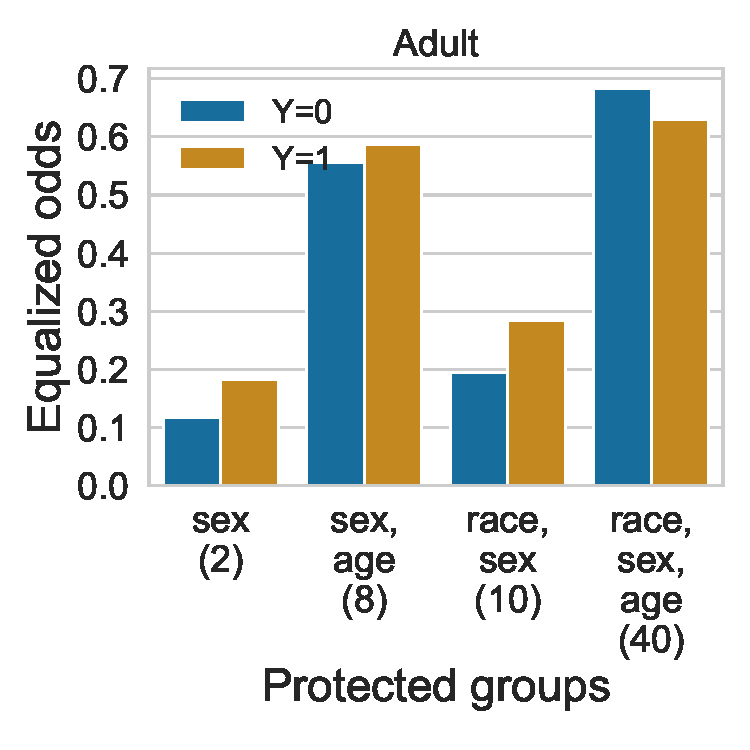
\includegraphics[scale=0.4]{figures/fairness/fvgm/sensitive_attribute_eqo_Adult_LR_Learn-efficient-dependency}}
		\subfloat{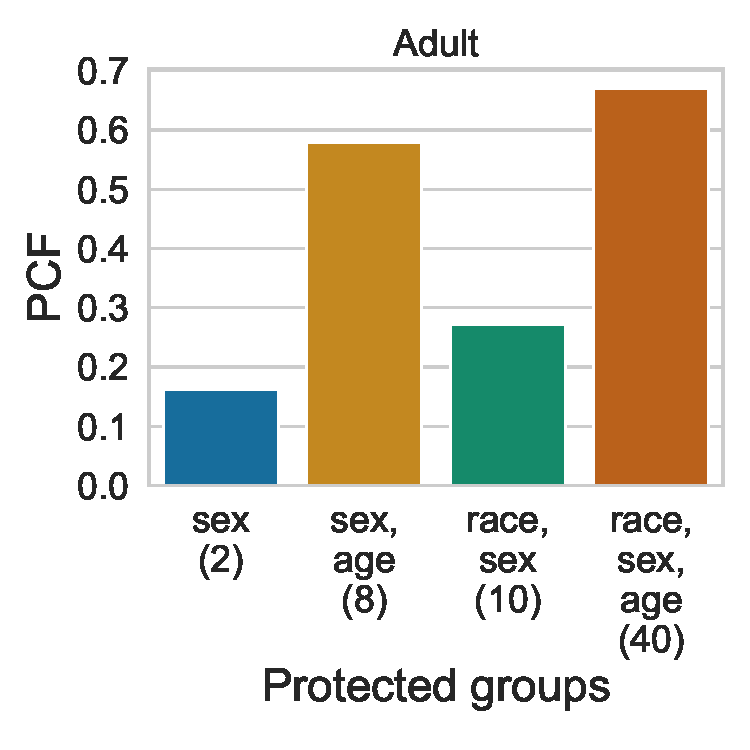
\includegraphics[scale=0.4]{figures/fairness/fvgm/sensitive_attribute__PCF_Adult_LR_Learn-efficient-dependency}}	
		\vspace{-1em}
		
		\subfloat{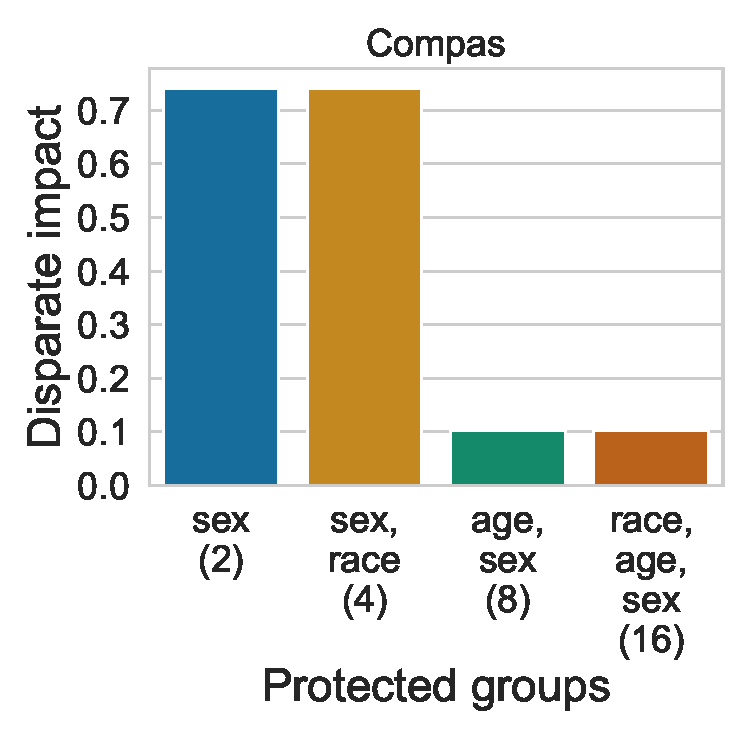
\includegraphics[scale=0.4]{figures/fairness/fvgm/sensitive_attribute__Disparate_impact_Compas_LR_Learn-efficient-dependency}}			
		\subfloat{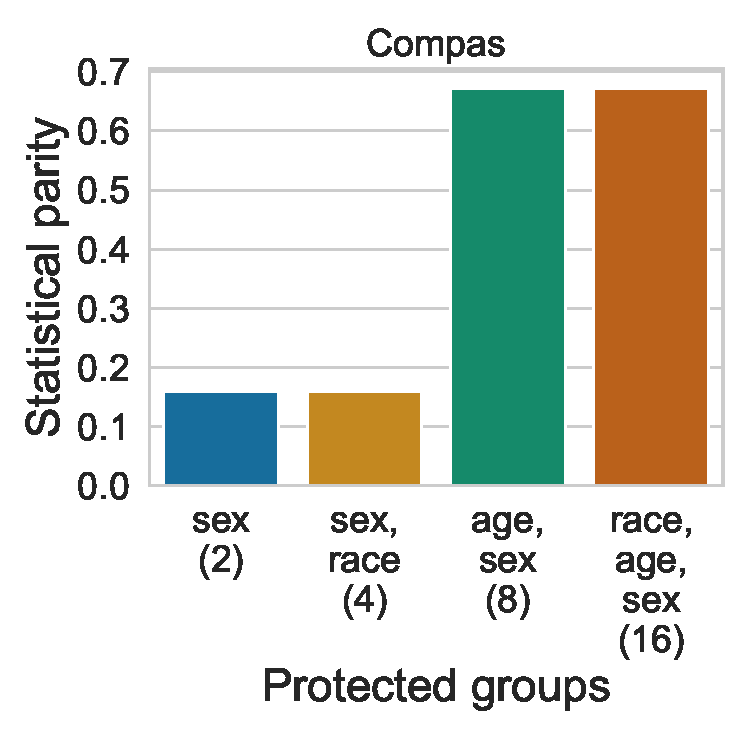
\includegraphics[scale=0.4]{figures/fairness/fvgm/sensitive_attribute__Statistical_parity_Compas_LR_Learn-efficient-dependency}}
		\vspace{-1em}
		
		\subfloat{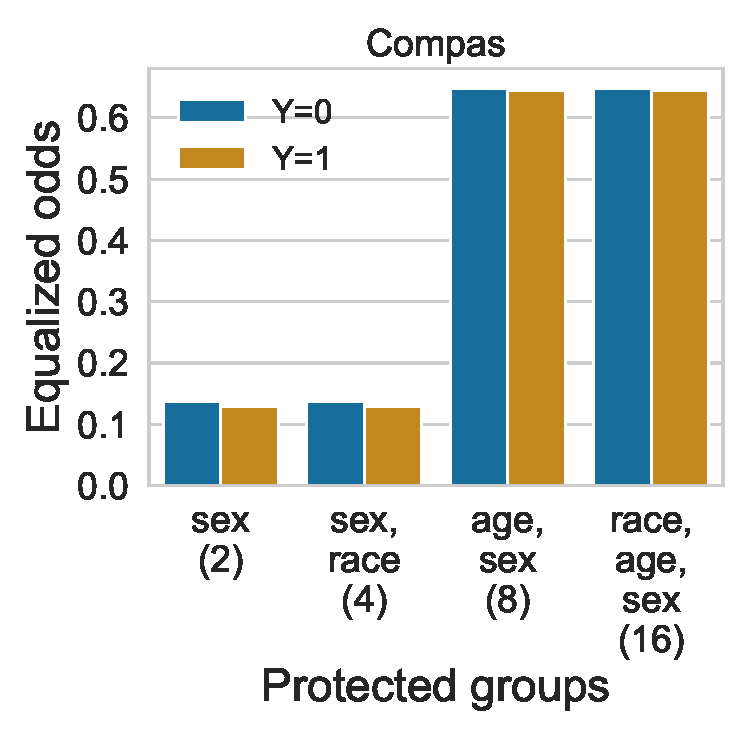
\includegraphics[scale=0.4]{figures/fairness/fvgm/sensitive_attribute_eqo_Compas_LR_Learn-efficient-dependency}}
		\subfloat{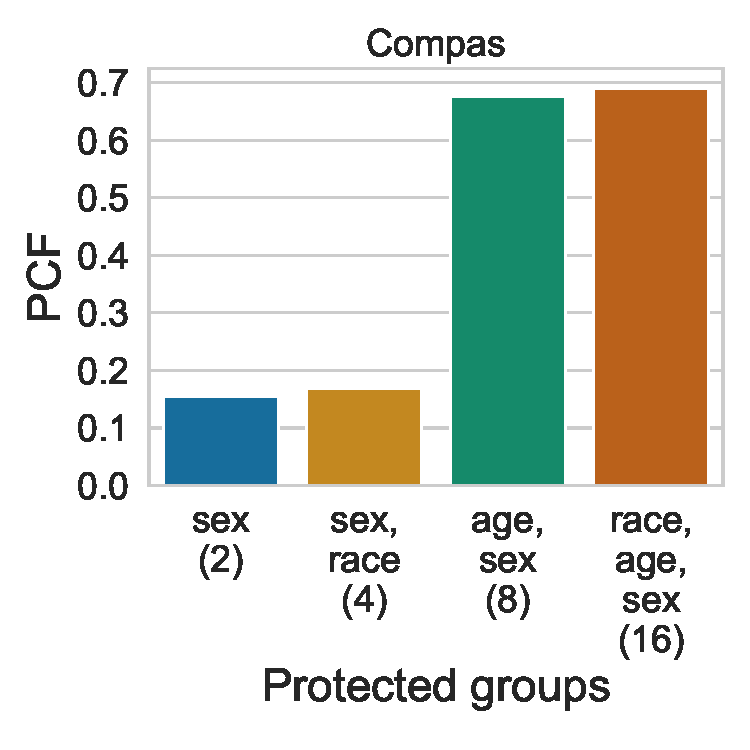
\includegraphics[scale=0.4]{figures/fairness/fvgm/sensitive_attribute__PCF_Compas_LR_Learn-efficient-dependency}}	
		
	\end{center}
		\caption{Verifying compound sensitive groups with respect to multiple fairness metrics. In each plot, the $ X $-axis shows sensitive features with the number of compound groups (within parenthesis) and $ Y $-axis shows computed group and causal fairness metrics. }
		\label{fairness_fvgm_fig:multiple_metrics}

\end{figure}
	
	
	
	
	\begin{figure}
		\begin{center}		
	
	\subfloat{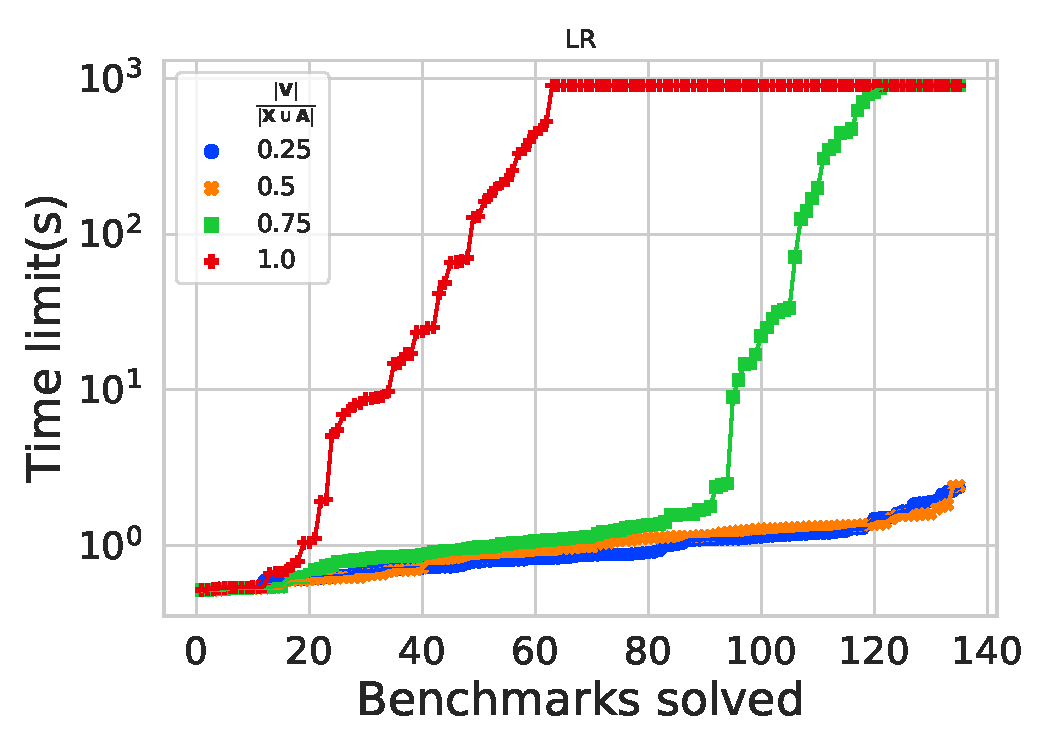
\includegraphics[scale=0.4]{figures/fairness/fvgm/cactus_dag_LR_time}}
	\subfloat{\includegraphics[scale=0.4]{figures/fairness/fvgm/cactus_dag_LR_time_notears}}
			
		\end{center}
		
		\caption[Ablation study: effect of Bayesian network on {\fvgm}]{Effect of number of variables in the learned Bayesian Network on computation time of {\fvgm}. In both plots, we vary $ \frac{|\mathbf{V}|}{|\nonsensitive \cup \sensitive|} $, that is the ratio between the number of variables in the Bayesian Network to the number of features. We observe that as this ratio increases to $ 1 $, both runtime of {\fvgm} (left plot) and network learning time (right plot) increase. } 
		\label{fairness_fvgm_fig:results_DAG_complexity}
\end{figure}
	
	
	

		
	\subsection{Verifying Fairness Algorithms on Multiple Fairness Metrics}
	
	We show extended results on verifying fairness attack in Figure~\ref{fig:attack_extended} for two fairness metrics: disparate impact (DI) and statistical parity (SP). We observe that {\framework} can detect poisoning attack for both metrics. 
	
	In Figure~\ref{fig:multiple_metrics} we show verification results on compound sensitive groups with respect to multiple fairness metrics. In this figure, we observe that with an increase in the number of groups, fairness metrics worsens\textemdash disparate impact decreases and other three metrics increases. Additionally, in Table~\ref{fig:extended_verifying_fairness_algorithms}, we show extended results for German and COMPAS dataset on verifying fairness algorithms: reweighing and optimized pre-processing algorithms. 
		
	\subsection{Performance Analysis of Bayesian Network}
	In Figure~\ref{fig:results_DAG_complexity}, we analyze the performance of encoding Bayesian Networks of differing complexity. We define the complexity of the network as  $ \frac{|V|}{|\nonsensitive \cup \sensitive|} $, which is the ratio between the number of features appearing in the network and total features. In this figure, as the ratio increases, both computation time of {\framework} and learning time of Bayesian Network increase. 
	
	
	
	\begin{table}[!t]
	
	\centering
	\small
	\caption{Extended results for verification of different fairness enhancing algorithms using {\framework}. Numbers in bold refer to fairness improvement w.r.t. different fairness metrics. RW and OP refer to reweighing and optimized-preprocessing algorithms respectively.  }
	\label{fig:extended_verifying_fairness_algorithms}
	\setlength{\tabcolsep}{.5em}
	
	\begin{tabular}{lllrrrrrrrrrrrrr}
		
		\toprule
		Dataset & Sensitive & Algo. & $ \Delta $DI &  $ \Delta $PCF & $ \Delta $SP & $ \Delta$ EO\\
		\midrule
		
		
		\multirow{4}{*}{Adult}&\multirow{2}{*}{race}&RW&$ \textbf{0.53} $&$ \textbf{-0.06} $&$ \textbf{-0.06} $&$ \textbf{-0.02} $\\
		&&OP&$ \textbf{0.57} $&$ \textbf{-0.07} $&$ \textbf{-0.07} $&$ \textbf{-0.02} $\\
		\cmidrule{2-7}
		&\multirow{2}{*}{sex}&RW&$ \textbf{0.96} $&$ \textbf{-0.16} $&$ \textbf{-0.15} $&$ \textbf{-0.08} $\\
		&&OP&$ \textbf{0.43} $&$ \textbf{-0.08} $&$ \textbf{-0.08} $&$ 0.03 $\\
		
		\midrule
		\multirow{4}{*}{COMPAS}&\multirow{2}{*}{race}&RW&$ \textbf{0.13} $&$ \textbf{-0.07} $&$ \textbf{-0.07} $&$ \textbf{-0.06} $\\
		&&OP&$ \textbf{0.15} $&$ \textbf{-0.08} $&$ \textbf{-0.08} $&$ \textbf{-0.05} $\\
		\cmidrule{2-7}
		&\multirow{2}{*}{sex}&RW&$ \textbf{0.1} $&$ \textbf{-0.04} $&$ \textbf{-0.04} $&$ 0.04 $\\
		&&OP&$ \textbf{0.09} $&$ \textbf{-0.04} $&$ \textbf{-0.04} $&$ \textbf{-0.03} $\\
		
		\midrule
		\multirow{4}{*}{German}&\multirow{2}{*}{age}&RW&$ \textbf{0.52} $&$ \textbf{-0.53} $&$ \textbf{-0.52} $&$ \textbf{-0.47} $\\
		&&OP&$ \textbf{0.53} $&$ \textbf{-0.53} $&$ \textbf{-0.53} $&$ \textbf{-0.51} $\\
		\cmidrule{2-7}
		&\multirow{2}{*}{sex}&RW&$ -0.06 $&$ 0.06 $&$ 0.06 $&$ 0.02 $\\
		&&OP&$ -0.12 $&$ 0.12 $&$ 0.12 $&$ 0.07 $\\
		
		
		\bottomrule
	\end{tabular}
\end{table}
	
	
	
\iffalse
\begin{table}[h!]
		\centering
		\caption{Extended results for runtime of different verifiers in seconds.  `\textemdash'~ refers to timeout ($ 900 $ seconds). Bold number refers to best scalability results. We additionally show results for decision tree classifiers (DT). {\framework} takes comparatively more time for decision tree classifiers because of encoding feature-correlations represented as a Bayesian network.}
			\label{tab:scalability_extended}	
		\begin{tabular}{llrrrrrrrrrrrrrr}
			
			\toprule
			Dataset & Classifier & FairSquare & VeriFair & Justicia & {\framework} \\
			\midrule
			
			\multirow{3}{*}{Ricci} & LR & \textemdash &  $ 2.0 $  &  $ 2.2 $  &  $ \textbf{0.1} $  \\ 
			& SVM & \textemdash &  $ 1.8 $  &  $ 2.2 $  &  $ \textbf{0.1} $  \\ 
			& DT &  $ 4.6 $  &  $ 1.9 $  &  $ \textbf{0.1} $  &  $ \textbf{0.1} $  \\ 
			
			
			\midrule
			\multirow{3}{*}{Titanic} & LR & \textemdash &  $ 0.5 $  &  $ 0.3 $  &  $ \textbf{0.1} $  \\ 
			& SVM & \textemdash &  $ 0.4 $  &  $ 0.2 $  &  $ \textbf{0.1} $  \\ 
			& DT &  $ 432.9 $  &  $ 17.2 $  &  $ \textbf{0.3} $  &  $ 1.6 $  \\ 
			
			
			\midrule
			\multirow{3}{*}{Compas} & LR & \textemdash &  $ 12.2 $  & \textemdash &  $ \textbf{0.4} $  \\ 
			& SVM & \textemdash &  $ 11.6 $  & \textemdash &  $ \textbf{0.5} $  \\ 
			& DT & \textemdash &  $ 377.1 $  &  $ \textbf{0.3} $  &  $ 121.7 $  \\ 
			
			
			\midrule
			\multirow{3}{*}{Adult} & LR & \textemdash &  $ 7.3 $  & \textemdash &  $ \textbf{0.9} $  \\ 
			& SVM & \textemdash &  $ 21.7 $  &  $ \textbf{1.7} $  &  $ 1.8 $  \\ 
			& DT & \textemdash &  $ 57.9 $  &  $ 0.4 $  &  $ \textbf{0.3} $  \\ 
			
			
			\midrule
			\multirow{3}{*}{German} & LR & \textemdash &  $ 19.2 $  & \textemdash &  $ \textbf{1.4} $  \\ 
			& SVM & \textemdash &  $ 28.8 $  & \textemdash &  $ \textbf{1.4} $  \\ 
			& DT & \textemdash &  $ 78.5 $  &  $ \textbf{0.2} $  &  $ 2.3 $  \\ 
			
			
			\bottomrule
			
			
		\end{tabular}
		
	\end{table}	
\fi		

%\newpage
%\clearpage
\section{Fairness Influence Functions (FIF)}
Now, we present an elaborate discussion on computing fairness influence functions.
A Fairness Influence Function, denoted as $ \mathsf{FIF}(\cdot) $, is computed with respect to a \textit{quantity of interest}, for example, the  PPV of the classifier or different fairness metrics such as DI and SP. Let $ \mathbf{S}  \subseteq \nonsensitive $ be a set of non-sensitive features, for which we are interested in computing their influence. A general approach to compute $ \mathsf{FIF}(\mathbf{S}) $ is to replace each feature in $ \mathbf{S} $ with random values and report differences in the quantity of interest~\cite{datta2016algorithmic}. Let $ \mathcal{X}'_i $ denote the modified marginal distribution where we replace feature $ X_i \in \mathbf{S} $ with random values. For example, $ \mathcal{X}'_i $ can be viewed as an uniform distribution within the support of $ X_i $. We then define the modified product distribution, denoted as $ \mathcal{D}_{-\mathbf{S}} $ by combining all marginal distributions, where each feature in $ \mathbf{S} $ has a modified distribution. 
\[
\mathcal{D}_{-\mathbf{S}} = \prod_{i | X_i \in \mathbf{S}} \mathcal{X}'_i \prod_{i | X_i \in X \setminus \mathbf{S}} \mathcal{X}_i \prod_{j=1}^{n} \mathcal{A}_j 
\]
We first give a general definition of influence function of $ \mathbf{S} $ on a quantity, say $ Q $, in the following. 
\[
\mathsf{FIF}(\mathbf{S}) \triangleq Q(\mathcal{D}) - Q(\mathcal{D}_{-\mathbf{S}})
\]
Intuitively, influence of $ \mathbf{S} $ is the difference in a quantity computed for the original distribution $ \mathcal{D} $ and the modified distribution $ \mathcal{D}_{-\mathbf{S}} $. In the following, we define influence function in terms of PPV of the classifier. 
\[
\mathsf{FIF}_{\mathsf{PPV}}(\mathbf{S}) \triangleq \Pr[\hat{Y} = 1 | \mathcal{D}] - \Pr[\hat{Y} = 1 | \mathcal{D}_{-\mathbf{S}}]
\]
Influence function also generalizes to PPV specific to compound sensitive groups. For a sensitive group $ \mathbf{a} \in \sensitive $, we define group-specific influence as follows. 

\[
\mathsf{FIF}_{\mathsf{PPV},\; \mathbf{a}}(\mathbf{S}) \triangleq \Pr[\hat{Y} = 1 | \sensitive = \mathbf{a}, \mathcal{D}] - \Pr[\hat{Y} = 1 | \sensitive = \mathbf{a},  \mathcal{D}_{-\mathbf{S}}]
\]

\paragraph{Experimental Analysis.} We empirically instantiate computation of FIF and its consequences for a logistic regression classifier on COMPAS and Adult datasets.

For both the datasets, we consider biological `sex' as the sensitive features.
In both cases, we denote the sensitive groups `male' and `female' as `sex=0' and `sex=1', respectively. 
FIFs computed for these sensitive groups show influence of different features and their relevant disparities. We illustrate the results in Figure~\ref{fairness_fvgm_fig:fif}.

Figure~\ref{fairness_fvgm_fig:fif_a} illustrates that the PPV value for the `male' population in the dataset is $0.61$. If we now replace the feature `age' with uniformly random values, the PPV for the same group becomes $0.46$, Thus, the FIF of the feature `age' for `male' group is $0.15$.
Similarly, all the red bars in Figures~\ref{fairness_fvgm_fig:fif_a}-\ref{fairness_fvgm_fig:fif_b}, ~\ref{fairness_fvgm_fig:fif_c}-\ref{fairness_fvgm_fig:fif_d} indicate a positive influence of that feature and the green bars indicate a negative influence of the feature on the individual getting classified to $\hat{Y}=1$.

In Figures~\ref{fairness_fvgm_fig:fif_c} and~\ref{fairness_fvgm_fig:fif_f}, we illustrate the influence of different features on the disparate impact between the two groups `male' and `female'. 
The green bar indicates that removing a feature causes an increase in DI, i.e. fairness in classification, and the red bar indicates the opposite. Alternatively, we can conclude that bigger is the green bar for a feature, higher is the bias-inducing effect of it.

Thus, from Figure~\ref{fairness_fvgm_fig:fif_c}, we conclude that `age' is the most bias-inducing feature among the two groups `male' and `female'.
From Fig~\ref{fairness_fvgm_fig:fif_a} and~\ref{fairness_fvgm_fig:fif_b}, we observe that `age' is a decisive feature for `male' while it is comparatively insignificant for `female'.

In case of Adult dataset, the PPV for `male' and `female' groups are 0.45 and 0.3 respectively. Among all the features, we observe that `race' has a positive impact on the classification for both the groups. This means removing the `race' information decreases the chance of getting classified to higher economic group. On the other hand, `capital-gain' has the highest influence on the classification for both groups. It is also the most biased-inducing feature as it varies most disparately among the two groups as the `capital-gain' differs significantly between two groups. 
\begin{figure}
	\begin{center}
	
		\subfloat[COMPAS]{\includegraphics[scale=0.35]{figures/fairness/fvgm/dependency_exp_Learn-dependency_compas_lr_sex_0}\label{fairness_fvgm_fig:fif_a}}
		\subfloat[COMPAS]{\includegraphics[scale=0.35]{figures/fairness/fvgm/dependency_exp_Learn-dependency_compas_lr_sex_1}\label{fairness_fvgm_fig:fif_b}}\\
		\subfloat[Adult]{\includegraphics[scale=0.35]{figures/fairness/fvgm/dependency_exp_Learn-dependency_adult_lr_sex_0}\label{fairness_fvgm_fig:fif_d}}
		\subfloat[Adult]{\includegraphics[scale=0.35]{figures/fairness/fvgm/dependency_exp_Learn-dependency_adult_lr_sex_1}\label{fairness_fvgm_fig:fif_e}}\\
		\subfloat[COMPAS]{\includegraphics[scale=0.35]{figures/fairness/fvgm/dependency_exp_Learn-dependency_compas_lr_sex_DI}\label{fairness_fvgm_fig:fif_c}}
		\subfloat[Adult]{\includegraphics[scale=0.35]{figures/fairness/fvgm/dependency_exp_Learn-dependency_adult_lr_sex_DI}\label{fairness_fvgm_fig:fif_f}}\\
		
	
		
	\end{center}
	\caption[FIF illustration using {\fvgm}]{Extended results on computing feature influence functions (FIF) for COMPAS  and Adult dataset.}\label{fairness_fvgm_fig:fif}
\end{figure}





\iffalse
\clearpage
\paragraph{Limitations of existing SSAT solvers.}
Since there is no state of the art SSAT solver that can handle universal quantification, we cannot consider conditional probabilities of universal variables while encoding the Bayesian network. In {\framework}, universal quantification appears while learning the least favored group in the learning encoding. When we do not consider conditional probabilities on universal variables, earlier approach could solve this using an existential SSAT solver by first negating the CNF and then subtracting computed probability from $ 1 $ as a solution to the original universal SSAT problem. This approach does not work when conditional probabilities are involved. 

For example, consider a clause $ a \vee\mathbf{B}\vee c $ defined on three Boolean variables where $ a $ is existential and $ b,c $ are random. Without considering conditional probabilities on $ a $, it is assigned true trivially. However, with conditional probabilities $ a $ can be false depending on the probability. Similar argument holds when $ a $ is universal. Hence, when conditional probabilities are considered for universal variables, a dedicated SSAT solver is also required to solve them. 
\fi





%\noindent\makebox[\linewidth]{\rule{\textwidth}{0.4pt}}	



\iffalse
\clearpage

\section{Progress}

\begin{enumerate}
	\item \textbf{Encoding conditional probabilities:} In our experiments, we have studied two algorithms for learning Bayesian network from data: Notears and pgmpy. After learning a DAG structure, we post-process it before feeding to {\framework}. 
	
	\begin{itemize}
		\item \textbf{Modifying in-degree edges for sensitive variables.} In the SSAT-based encoding, sensitive variables have existential (or universal) quantification because we are interested in knowing which assignment to these variables result in the most (or least) favored group. 
		
		In a Bayesian network, a directed edge $ (a,b) $ between variable $ a $ and $\mathbf{B}$ refers to the conditional dependence of $\mathbf{B}$ on $ a $.  We now consider a case where variable $\mathbf{B}$ is a sensitive variable. Since an existential (or universal) quantification on variable $\mathbf{B}$ fixes its assignment, we first reverse the direction of the edge to $ (b,a) $ in order to capture the dependence between two variables. We highlight that {\framework} does not have a strict restriction for DAG structure as input. Therefore, even if reversing an edge may violate DAG structure, {\framework} is not affected by this modification. 
		
		If both $ a $ and $\mathbf{B}$ refers to different categories for a sensitive attribute, more specifically they belong to the one-hot encoded variables for a sensitive attribute, we remove the edge $ (a, b) $ from the learned DAG.  
		
		
		
		
	\end{itemize}
	
	\item \textbf{Verifying Path-specific Causal Fairness.}
	
	\item \textbf{Fairness Attack Verification:} We apply {\framework} to verify fairness poisoning attack \cite{?}. This attack algorithm generates poisoned data, which together with initial training data results in a ML classifier with decaying fairness results. With {\framework} we verify the effectiveness of fairness poisoning attacks.
	
	\item \textbf{Verifying pre-processing and post-processing fairness algorithms:} We apply {\framework} to verify the  effectiveness of fairness enhancing algorithms, in particular pre-processing and post-processing algorithms. 
	
	\begin{itemize}
		\item \textbf{Pre-processing fairness algorithms.} Pre-processing algorithms process a  dataset such that any model learned on the dataset has better fairness results, computed in terms of disparate impact, statistical parity and so on. To verify the effectiveness of a pre-processing algorithm, we first train a classifier on unprocessed data and later another classifier on processed data. Finally, we compute the difference in different fairness metrics using {\framework}. For an effective fairness algorithm, disparate impact increases and statistical parity decreases for the processed data.  
		
		\item \textbf{Post-processing fairness algorithms.} 
		Post processing fairness algorithms works on the output of any already trained classifier so that the final output by the fairness algorithm improves fairness of the classifier. \red{In order to verify a post-processing fairness algorithm, we learn a new classifier on the processed data\footnote{Learning a new classifier is not a requirement for approaches that can compute fairness on a dataset (includes class-label). However, our framework requires a classifier, which learns the mapping between input features and class-label. } and report difference in fairness metrics. The new classifier should have high accuracy on the processed data, otherwise the verification result by {\framework} is not reliable.  }
		
	\end{itemize}
	
	\item \textbf{Feature Influence.} We employ {\framework} to compute feature-influence of each feature in the data. For a distribution $ \mathcal{D} $, a finite sample dataset $ D \sim \mathcal{D} $, and feature $ x $, we define its influence in terms of the positive predictive value (PPV) of the classifier.  
	\[
	q(x) \triangleq  \Pr[\hat{Y}_{D_{-x}} = 1 | \mathcal{D}_{-x}] - \Pr[\hat{Y}_D = 1 | \mathcal{D}]
	\]
	
	In this equation, $ \mathcal{D}_{-x} $ (resp.\ $ D_{-x} $) refers to the distribution (resp.\ dataset) where all but feature $ x $ are present.
	Intuitively, the influence of feature $ x $ is the difference in positive predictive value of the classifier as if $ x $ does and does not participate in the task of classification. Note that, the classifier is learned on dataset $ D $ whereas $ q(x) $ is computed for the distribution $ \mathcal{D} $.
	
	\textbf{Outline:}
	\begin{enumerate}
		\item Train a classifier $ M $ on a dataset $ D $
		\item From the dataset, compute product distribution of features $ \mathcal{D} $. This is handled by {\framework} \red{Can we implement an interface where the distribution is passed as inputs? }
		\item Compute base values of different fairness metrics. In our experiments, we have computed disparate impact and statistical parity. '
		\item To compute the influence of an attribute, we replace that attribute with random value on the dataset $ D' $. For a continuous attribute, we randomly generate attribute value within the maximum and minimum of original attribute-values. For a categorical attribute, we randomly select a category. 
		\item We again calculate distribution from $ D' $ and run {\framework} on the new distribution.
		\item Since random-value replacement involves randomness, we have repeated the process for $ 5 $ iterations. 
	\end{enumerate}
	
	\textbf{Result Analysis}
	We first learn dependency among features using Bayesian structure learning algorithm. For the dependency structure, we compute feature-influence and report in Figure~\ref{fig:feature_influence_compas}. In COMPAS dataset, we consider `race' as a sensitive attribute where race = 1 denotes Caucasian. In all three reported classifiers, prior-counts and juvenile-count are top influential features for both sensitive group. Other non-crime features such as race, age are also found to be influential for logistic regression classifier and CNF classifier. Moreover, depending on sensitive group, age and race have differentiating influence. 
	\red{Incomplete analysis}
	
\end{enumerate}	



For the learning encoding, sensitive variables $ \sensitive $ are existentially quantified in $ \mathsf{prefix_{ERE}} $ and universally quantified in $ \mathsf{prefix_{URE}} $. These variables are followed by randomized quantified variables $ \lambda_{X_i}, \lambda_{x,\mathbf{u}} $ and $ X_j \in \nonsensitive \setminus V $. Finally, remaining variables such as $ \lambda_{\hat{Y}} $ and $ X_i $ for each $ X_i \in V(G) $ are existentially quantified. 


\paragraph{Extra}
To this end, we consider all features $ \nonsensitive \cup \sensitive $ to be Boolean. We additionally constrain the classifier $ \hat{Y} $  to be a Boolean formula $ \phi_{\hat{Y}} $ in CNF defined over $ \nonsensitive \cup \sensitive $ such that, for an assignment of $ \nonsensitive \cup \sensitive $, $ \hat{Y} = 1 $ whenever $ \phi_{\hat{Y}} $ is true, and $ \hat{Y} = 0 $ otherwise. Additionally, we construct another CNF formula $ \phi_\BN $ to encode the joint distribution of $ \BN $, which we discuss shortly.

One approach to verify different fairness metrics such as disparate impact, statistical parity, equalized odds, and path-specific causal fairness is to compute the most favored group and the least favored group based on the group specific PPV of the classifier~\cite{ghosh2020justicia}. As such, we can either (i) enumerate computation of group specific PPV for all sensitive groups or (ii) learn the most favored group and the least favored group, to compute these metrics. 	Provided that we have  $ \phi_{\hat{Y}} $ and $ \phi_\BN $ representing the classifier and the Bayesian network, we now discuss two encodings in the following. 

\begin{enumerate}
	\item \textbf{Enumeration.} We consider an RE-SSAT (Randomized Exponential Stochastic SAT) instance with random quantifier over Boolean variables to compute $ \Pr[\hat{Y} = 1 | \sensitive = \mathbf{a}, \BN] $. 
	\begin{align}
	\Phi_{\mathbf{a}} = \mathsf{prefix_{Enum}}, \phi_{\hat{Y}} \wedge \phi_\BN \wedge (\sensitive = \mathbf{a})
	\end{align}
	where $ \mathsf{prefix_{Enum}} $ is an ordered sequence of randomized quantified Boolean variables and $ \sensitive = \mathbf{a} $ encodes the sensitive group $ \mathbf{a} \in \sensitive $ as a CNF. We discuss quantifiers in detail in Section~\ref{?}. An RE-SSAT formula can be solved by a projected model counter where we project model-counting (number of satisfying assignments in a CNF) on randomized quantified variables. Solving $ \Phi_{\mathbf{a}} $,  the probability of satisfaction $ \Pr[\Phi_{\mathbf{a}}] $ exactly computes group-specific PPV of the classifier, $ \Pr[\hat{Y} = 1 | \sensitive = \mathbf{a}, \BN] $. Finally, we enumerate this computation for all sensitive groups $ \forall \mathsf{a} \in A $ and use  $ \max_{\mathbf{a}} \Pr[\Phi_{\mathbf{a}}] $  and $ \min_{\mathbf{a}} \Pr[\Phi_{\mathbf{a}}] $\textemdash the PPV of the most and the least favored group, respectively\textemdash  to compute different fairness metrics. 
	
	
	\item \textbf{Learning.} The second encoding efficiently learns the most favored group and the least favored group by instantiating two SSAT formulas: ERE (Existential-Random-Existential) and URE (Universal-Random-Existential) SSAT formulas, respectively. Both SSAT formulas have the same CNF formula and only difference is in the prefix. 
	\begin{align}
	&\Phi_\mathsf{ERE} = \mathsf{prefix_{ERE}}, \phi_{\hat{Y}} \wedge \phi_\BN\\
	&\Phi_\mathsf{URE} = \mathsf{prefix_{URE}}, \phi_{\hat{Y}} \wedge \phi_\BN
	\end{align}
	$ \mathsf{prefix_{ERE}} $ (resp.\ $ \mathsf{prefix_{URE}} $) is an ordered sequence of existentially (resp.\ universally) quantified variables followed by randomized quantified variables.
	We apply existential quantifier ($ \exists $) on sensitive features $ A $ in $ \Phi_\mathsf{ERE} $ using $ \mathsf{prefix_{ERE}} $. Therefore, according to rule(??) in Section\ref{??}, we learn an assignment to $ A $, say the most favored sensitive group,  resulting in the maximum satisfying probability of $ \Phi_\mathsf{ERE} $. Formally, $ \Pr[\Phi_\mathsf{ER}] $ is equal to $ \max_{\mathbf{a}} \Pr[\Phi_{\mathbf{a}}] $ in the enumeration encoding. We similarly apply universal quantifiers ($ \forall $) on $ A $ to learn the least favored sensitive group with $ \Pr[\Phi_\mathsf{URE}] $ equalizing to $ \min_{\mathbf{a}} \Pr[\Phi_{\mathbf{a}}] $. 
\end{enumerate}

\red{Complexity analysis has to be verified.}
Both enumeration and learning encoding output same results and their worst case complexity is same. In particular, solving an  RE-SSAT formula has complexity $ \text{PP}^{\text{NP}} $ and we enumerate for all sensitive groups, which is exponentially many in $ A $. Similarly, solving both ER-SSAT and URE-SSAT is $ \text{NP}^{\text{PP}} $ hard.

We now discuss the construction of the CNF formula, particularly $ \phi_{\hat{Y}} $ and $ \phi_\BN $. Ghosh et al.~\cite{ghosh2020justicia} have proposed techniques to encode decision trees and linear classifiers as a CNF formula $ \phi_{\hat{Y}} $. For linear classifiers, the decision function is viewed as a pseudo-Boolean constraint and can be efficiently encoded to CNF by introducing auxiliary variables, denoted by $ \lambda_{\hat{Y}} $.  Support-vector classifiers with linear kernels can also be encoded to CNF in the same approach to linear classifiers. Hence, we now focus on the construction of $ \phi_\BN $ to encode the Bayesian network to CNF.








\red{Additional}
\begin{enumerate}
	\item Advance terminate when $ S(W,\tau, Q) \le w_{neg} $, where $ w_{neg} $ is the sum of negative weights in $ W $.
	\item Within similar quantifiers, sort based on descending weights to leverage early termination.
	\item We can learn maximum and minimum of $ S(W,\tau,Q) $ in one go (should be explained in dynamic programming). It is not required to convert weights to positive. One benefit of assuming all positive weights is that we then have one sub-problem with selection of weights (and this sub-problem has maximum value). However, to compute minimum of $ S $, we again need to consider the sub-problem with not selection of weights. But we can propose a dynamic approach where both max and min can be solved in one go. 
\end{enumerate}






\section{Experimental Evaluations}






\begin{figure}
	\begin{center}
		\subfloat[]{\includegraphics[scale=0.4]{figures/BN_Edges}}
		\subfloat[]{\includegraphics[scale=0.4]{figures/BN_Time_(DAG)}}\\
		\subfloat[]{\includegraphics[scale=0.4]{figures/BN_Disparate_impact}}
		\subfloat[]{\includegraphics[scale=0.4]{figures/BN_Statistical_parity}}\\
		\subfloat[]{\includegraphics[scale=0.4]{figures/BN_ppv}}\\
	\end{center}
	\caption{Experimenting the effect of regularizer in DAG learner inside {\framework}. With increasing values of regularizer, learned DAGs become sparser by undertaking less learning time. For different DAGs, we evaluate positive predictive value (PPV) for a fixed classification algorithm. We occasionally observe that disparate impact  increases and statistical parity decreases for sparser DAG. We show break down result for two different sensitive groups where the group `Age $ = 1 $' is often (but not always) more discriminated than `Age $ = 0 $'  in majority values of regularizer.  Therefore, {\framework} can verify bias induced by data (in form of Bayesian Network)  for the fixed classification algorithm.}
\end{figure}
\fi


	%	\newpage





\section{Fairness Verification of CNF Classifiers with Feature-correlations} 
\label{sec:CNF_feature_correlation}
Existing verifiers such as Justicia focuses mainly on classifiers expressible as a CNF formula. But none of the existing verifiers consider correlation among the features while computing fairness metrics. In this section,  we address fairness verification of CNF-based classifiers with explicit consideration of correlations among features. In particular, we present how to encode a Bayesian network, which captures correlated features, into a SSAT-based formulation that is tailored for verifying CNF classifiers. To this end, we first discuss the basics of SSAT followed by an elaboration of the proposed methodology.



\subsection{Background: Stochastic Boolean Satisfiability (SSAT)}\label{sec:ssat}
Let $ \mathbf{B}  = \{\bool_1, \dots, \bool_m\}  $ be a set of Boolean variables taking assignment in $ \{0,1\}^m $. A \textit{literal} $ l_i $ is a variable $ \bool_i $ or its complement $ \neg \bool_i $. A propositional formula $\phi$ defined over $\mathbf{B}$ is in CNF if $\phi \triangleq \wedge_i C_i $   is  a conjunction of clauses and each clause $ C_i \triangleq \vee_j l_j $ is a disjunction of literals. A CNF formula $ \phi $ is satisfied (called SAT) if there is an assignment $ \sigma $ over $\mathbf{B}$ that evaluates formula $ \phi $ to $ 1 $ (or true)\textemdash at least one literal in each clause is true and all clauses are true. We additionally consider a quantification over each Boolean variable $ B_i $, denoted by $ q_i \in \{\exists, \forall, \R^{p_i}\}$, where $ \exists $ is existential, $ \forall $ is universal and $ \R $ is a randomized quantifier with $ p_i = \Pr[B_i = 1] $. The SSAT problem takes \textit{an ordered set of quantifiers} over  $\mathbf{B}$ and a CNF formula $ \phi $ and computes the \textit{probability of satisfaction} of $ \phi $ given quantifiers.  Formally, a SSAT formula $ \Phi \triangleq (\{q_i\}_{i=1}^{m}, \phi) $ and the SSAT problem computes $ \Pr[\Phi]  \in [0,1]$. The semantics of SSAT formula is in the following.

\begin{enumerate}
	\item $ \Pr[\text{true}] = 1 $,  $ \Pr[\text{false}] = 0 $, 
	\item $ \Pr [\Phi] = \max_{\bool_1} \{\Pr[\Phi|_{\bool_1}], \Pr[\Phi|_{\neg \bool_1}]\}$ if $ \bool_1 $ is existentially quantified ($ \exists $), 
	\item $ \Pr [\Phi] = \min_{\bool_1} \{\Pr[\Phi|_{\bool_1}], \Pr[\Phi|_{\neg \bool_1}]\} $ if $ \bool_1 $ is universally quantified ($ \forall $), 
	\item $ \Pr [\Phi] = p\Pr[\Phi|_{\bool_1}] + (1-p) \Pr[\Phi|_{\neg \bool_1}] $ if $ \bool_1 $ is randomized quantified ($\R^{p}$) with probability $p = \Pr[\bool_1 = 1]$,
\end{enumerate}

In SSAT, we recursively solve for each Boolean variable in $\mathbf{B}$ starting with the first variable $ B_1 $
where $ \Phi|_{\bool_1} $ (resp.\ $ \Phi|_{\neg \bool_1} $) is the SSAT formula with CNF $ \phi $ substituted by an assignment of $ \bool_1 $ as true (resp.\ false) and quantifiers $ \{q_i\}_{i=2}^{m} $. 	

In this paper, we are interested in two specific SSAT formulations: exists-random (ER) SSAT formulas and universal-random (UR) SSAT formulas. In ER-SSAT (resp.\ UR-SSAT), $ \{q_i\} $ is constructed such that  existential (resp.\ universal) quantified variables is followed by randomized quantified variables. For more details on SSAT formulas,  we refer to \cite{ghosh2020justicia,lee2017solving, lee2018solving}.

%This correspondence of existential and universal quantifiers of choice variables with the maximum and minimum probabilities in case of SSAT, motivate us to assign the choice (or sensitive) variables similar quantifiers while computing the maximum and minimum PPVs for linear classifiers.






\subsection{Methodology}
For CNF classifiers~\cite{GMM20}, SSAT is a natural choice as it computes the probability of a CNF formula  given quantifiers of variables\textemdash equivalently, the PPV of a CNF classifier. \cite{ghosh2020justicia} has proposed a SSAT based formulation for verifying a CNF classifier $ \phi_{\hat{Y}} $ with a fundamental limitation of ignoring feature-correlations, which we address now. Let $ \phi_\BN $ be a CNF formula that encodes the Bayesian Network $ \BN $. Following~\cite{ghosh2020justicia}, we discuss an encoding that compute the PPV of the classifier for the most favored sensitive group with additional consideration of features-correlation. Let $\mathbf{Q}$ denote an ordered set of quantifiers over variables in the conjoined CNF $ \phi_{\hat{Y}} \wedge \phi_\BN $. We then construct a SSAT formula $ \Phi =  (\mathbf{Q},  \phi_{\hat{Y}} \wedge \phi_\BN) $ and solve it for computing $ \max_{\mathbf{a}} \Pr[\hat{Y} = 1 | \sensitive = \mathbf{a}] $. For computing $ \min_{\mathbf{a}} \Pr[\hat{Y} = 1 | \sensitive = \mathbf{a}] $ for the least favored group ,only difference is in the construction of $\mathbf{Q}$. We next discuss the construction of both $ \phi_\BN $ and $\mathbf{Q}$.





\paragraph{Encoding a Bayesian Network as a CNF Formula.}\label{sec:BN_to_CNF}
Our goal is to encode the Bayesian network $ \BN = (\graph, \factors) $ into a CNF formula $ \phi_\BN $ such that \textit{the weighted model count} of $ \phi_\BN $ exactly computes a joint probability distribution~\cite{chavira2008probabilistic}.  We note that SSAT does not allow conditional probabilities of randomized quantified variables trivially. Hence, $ \phi_\BN $ contains \textit{additional variables} to capture the conditional probabilities, as discussed next.


Let  $ G = (\mathbf{V}, E) $ where $  $  $ \mathbf{V} \subseteq \nonsensitive \cup \sensitive $ and $ \mathbf{E} \subseteq \mathbf{V} \times \mathbf{V} $. 	For each network variable $ V_i \in \mathbf{V} $, we define a Boolean \textit{indicator}  variable $ \lambda_{V_i} $ such that $ \Pr[\lambda_{V_i}] \triangleq \Pr[V_i] $. We add following constraint in $ \phi_\BN $ to establish the relation between $ \lambda_{V_i} $ and $ V_i $. 
\begin{align}
	\lambda_{V_i} \leftrightarrow V_i,
	\label{eq:indicator_constraint}
\end{align}
Intuitively, both $ \lambda_{V_i} $ and $ V_i $ are either true or false. This constraint can be trivially translated to clauses in CNF using the equivalence rule $ a \leftrightarrow b\equiv (\neg a \vee b)  \wedge (a \vee \neg a) $ for Boolean variables $ a, b$.

We now show encoding of conditional probabilities induced by parameter $ \theta $. Let $ V_i \in  \mathbf{V}  $  be a vertex in $ G $ where $ \parent(V_i) \ne \emptyset $ be $ V_i $'s parents and $ |\parent(V_i)| = k $. Additionally, let $ v $ and $ \mathbf{u} \triangleq [u_1,.., u_k] $ be an assignment of  $ V_i $ and $ \parent(V_i)  $, respectively.  To encode $ \Pr[V_i = v| \parent(V_i) = \mathbf{u}]$, we introduce auxiliary variable $ \lambda_{v,\mathbf{u}} $ and add following constraints in $ \phi_{\BN} $.
\begin{align}
	\lambda_{v,\mathbf{u}}  \wedge \bigwedge_{j=1}^{k} \lambda_{u_j} \rightarrow \lambda_v
	\label{eq:factor_pos}
\end{align}
\begin{align}
	\neg \lambda_{v,\mathbf{u}}  \wedge \bigwedge_{j=1}^{k} \lambda_{u_j} \rightarrow \neg \lambda_v
	\label{eq:factor_neg}
\end{align}

where $ \lambda_v \equiv \lambda_{V_i} $. Moreover, $ \lambda_{u_j} $ is the indicator variable corresponding to the $ j^\text{th} $ parent in $ \parent(V_i) $. In the above two constraints,	for a fixed assignment $ \mathbf{u} $ of parents $ \parent(V_i) $, both $ \lambda_v $ and $ \lambda_{v,\mathbf{u}} $ are either true or false.  Hence, these two constraints encode the conditional probability of $ V_i = v $ given $ \parent(V_i) = \mathbf{u} $ using $ \Pr[\lambda_{v,\mathbf{u}}] = \Pr[V_i = v| \parent(V_i) = \mathbf{u}]$. Both constraints can be translated to CNF clauses trivially. For example, Eq.~\ref{eq:factor_pos} is translated as $ \neg \lambda_{v,\mathbf{u}}  \vee \bigvee_{j=1}^{k} \neg \lambda_{u_j} \vee \lambda_v $. We next analyze the complexity of $ \phi_\BN $ in terms of the number of variables and clauses.

\begin{lemma}
	For a Bayesian network $ \BN = (\graph, \factors) $ defined over $ n $ Boolean network variables, the encoded CNF formula $ \phi_\BN $ has $ n + |\factors| $  variables and $ 2(n + |\factors|) $ clauses. 
\end{lemma}
\begin{proof}
	Since the DAG in the Bayesian network has $ n $ vertices, we consider $ n $ indicator variables. Moreover, for encoding conditional probabilities, we consider $ |\theta| $ auxiliary variables where parameter $ \theta $ denotes the number of distinct conditional probabilities in the network. Hence, total variables in $ \phi_\BN $ is $ n + |\factors|  $.
	
	According to Eq.~\eqref{eq:indicator_constraint},~\eqref{eq:factor_pos},~\eqref{eq:factor_neg}, there are $2( n + |\theta|) $ clauses in $ \phi_\BN $ as discussed in Section~\ref{sec:BN_to_CNF}.
	
	
\end{proof}

\begin{figure}[!t]
	\begin{center}
		\subfloat[]{\includegraphics[scale=0.33]{figures/sanity_ppv_max_PPV_DT}}
		\subfloat[]{\includegraphics[scale=0.33]{figures/sanity_ppv_min_PPV_DT}}\\
		\subfloat[]{\includegraphics[scale=0.33]{figures/sanity_sample_size_DI_DT}}
		\subfloat[]{\includegraphics[scale=0.33]{figures/sanity_sample_size_SPD_DT}}
		
		
	\end{center}
	
	\caption{
		Computing PPV of Decision Tree (DT) classifiers using {\framework} and Justicia. {\framework} incorporates correlated features represented as a Bayesian network in Figure~\ref{fig:synthetic_bn}. We also present the effect of sample size on different fairness metrics such as DI and SP for DT classifier. }
	\label{fig:synthetic_results}
\end{figure}

\paragraph{Constructing Quantifiers $ \mathbf{Q} $.}
We now discuss the ordered set of quantifiers for a SSAT formula containing CNF $ \phi_{\hat{Y}} \wedge \phi_\BN $\textemdash the solution of which constitutes the maximum (minimum) PPV of a CNF classifier. $ \phi_{\hat{Y}} \wedge \phi_\BN $ contains four different variables : (i) sensitive variables $ \sensitive $, (ii) non-sensitive variables $ \nonsensitive $, (iii) indicator variables $  \lambda_{V_i} $, and (iv) auxiliary variables $ \lambda_{v,\mathbf{u}} $. Among them, (iii) and (iv) are associated with $ \phi_\BN $ and the rest for $ \phi_{\hat{Y}} $. For computing the maximum PPV of the classifier, we construct  an exists-random-exists (ERE) SSAT formula with quantifiers $\mathbf{Q}$ as follows: we set sensitive features $ \sensitive $ with existential quantifiers in the beginning of $ \mathbf{Q} $ followed by $  \lambda_{V_i}, \lambda_{v,\mathbf{u}} $ and $ X_j \in \nonsensitive \setminus \mathbf{V} $ with randomized quantifiers. Since sensitive variables are existentially quantified\textemdash similar to stochastic subset-sum problem\textemdash the solution of SSAT formula is maximized.
Finally, remaining variables appearing in the Bayesian network such as $ X_i \in \mathbf{V} $ are existentially quantified in $\mathbf{Q}$ as their assignment is fixed by indicator variables $ \lambda_{V_i} $. In contrast, for computing the minimum PPV of the classifier, we consider an universal-random-exists (URE) SSAT formula  where we set sensitive features $ \sensitive $ as universal quantifiers with all other quantifiers remaining same.


\iffalse
\subsection{Verifying Classifiers with Non-Boolean Features} {\framework} can verify beyond non-Boolean features. For binary decision tree classifiers, real-valued features are discretized in each node of the tree by comparing the feature against a constant threshold. Thus, each node constitutes a Boolean feature and the tree itself forms a CNF formula, as shown by~\cite{ghosh2020justicia}.
\fi








%\clearpage
%	\bibliographystyle{plainnat.bst}
%	\bibliography{ref.bib}
	








